\documentclass{article}
\usepackage[]{graphicx}
\usepackage[]{xcolor}
\usepackage{alltt}
\usepackage[left=2.3cm,right=2.8cm, top = 2.2cm, bottom = 3cm]{geometry}
\usepackage{amsmath}
\usepackage{amssymb}
\usepackage{natbib}
\PassOptionsToPackage{hyphens}{url}
\usepackage{url} 
\usepackage[disable]{todonotes}
\usepackage{multicol}
\usepackage{rotating}
\usepackage{booktabs}
\usepackage[colorlinks=false]{hyperref} 
\setlength{\parskip}{\baselineskip}%
\setlength{\parindent}{0pt}%
\urlstyle{same}
\usepackage{lineno}
\linenumbers
\bibliographystyle{apalike}

% to handle authorship footnotes as numbers:
\makeatletter
\let\@fnsymbol\@arabic
\makeatother

\newcommand{\ra}[1]{\renewcommand{\arraystretch}{#1}}
\newcommand{\changed}[1]{#1}

% to write the simulated as iid symbol: 
\newcommand{\distas}[1]{\mathbin{\overset{#1}{\kern\z@\sim}}}%


\begin{document}


\title{Transformations of forecasts for evaluation in an epidemiological context}
  \author{Nikos I. Bosse\thanks{Department of Infectious Disease Epidemiology, London School of Hygiene \& Tropical Medicine, London, United Kingdom} $^{,}$\thanks{Centre for the Mathematical Modelling of Infectious Diseases, London, United Kingdom} $^{,*}$, 
  Sam Abbott\footnotemark[1] $^{,}$\footnotemark[2]$ ^{}$, 
  Anne Cori\thanks{MRC Centre for Outbreak Analysis and Modelling, Department of Infectious Disease Epidemiology, School of Public Health, Imperial College London, London, United Kingdom} $^{}$, \\
  Edwin van Leeuwen\thanks{Department of Infectious Disease Epidemiology, London School of Hygiene \& Tropical Medicine, London, United Kingdom} $^{,}$\thanks{UK Health Security Agency, London, United Kingdom} $^{}$, 
  Johannes Bracher\thanks{Institute of Economic Theory and Statistics, Karlsruhe Institute of Technology, Karlsruhe, Germany} $^{}$, 
  Sebastian Funk\footnotemark[1] $^{,}$\footnotemark[2]$ ^{}$}



\maketitle
%\tableofcontents
\begin{abstract}
Forecast evaluation plays an essential role in improving forecasting models can help inform future decision making. In epidemiology, forecasts are often scored using the Weighted Interval Score (WIS) or the Continuous Ranked Probability Score (CRPS), which are a measure of absolute distance between forecast and observation. Infectious disease processes are commonly described in terms of the growth rate or the effective reproduction number. Scoring based on the absolute distance between forecast and observation may not reflect the true underlying modelling task well (estimating the growth rate or reproduction number) and makes it difficult to compare forecasts across time, space, and different targets. As a solution we propose transforming the data before scoring the forecasts. Depending on the context, many transformations may be appropriate. We describe the log-transformation as one specific example in detail and discuss its interpretation as a measure of relative error and as score for an implicit forecast of the exponential growth rate. Applying the log-transformation to data from the European COVID-19 Forecast Hub, we found that it changed model rankings, evened scores across time, locations and target types, and emphasised situations in which models missed lower inflection points and consequent rises in numbers, while penalising missed peaks less severely. 
\end{abstract}

\bigskip

{\footnotesize $^*$ Correspondence to \url{nikos.bosse@lshtm.ac.uk})}



\newpage


% ===========================================================
\section{Introduction}

Probabilistic forecasts \citep{heldProbabilisticForecastingInfectious2017} play an important role in decision-making in epidemiology and public health \citep{reichCollaborativeMultiyearMultimodel2019, funkShorttermForecastsInform2020, cramerEvaluationIndividualEnsemble2021, bracherShorttermForecastingCOVID192021, europeancovid-19forecasthubEuropeanCovid19Forecast2021, sherrattPredictivePerformanceMultimodel2022}, as well as other areas as diverse as economics \citep{timmermannForecastingMethodsFinance2018, elliottForecastingEconomicsFinance2016} or meteorology \citep{gneitingWeatherForecastingEnsemble2005, kukkonenReviewOperationalRegionalscale2012}. Epidemiological modelling in particular has received widespread attention during the COVID-19 pandemic. Evaluations of forecasts can provide feedback for forecasters and researchers to improve their models and train ensembles, and help decision makers distinguish good from bad predictions and choosing forecasters and models that should inform future decisions.

Probabilistic forecasts are usually evaluated using so-called proper scoring rules \citep{gneitingStrictlyProperScoring2007}, which return a numerical score as a function of the forecast and the observed data. Proper scoring rules are constructed such that forecasters are incentivised to report their true belief about the future. Examples of proper scoring rules that have been used to assess epidemiological forecasts are the Continuous Ranked Probability Score~\citep[CRPS,][]]{gneitingStrictlyProperScoring2007} or its discrete equivalent, the Ranked Probability Score~\citep[RPS,][]{funkAssessingPerformanceRealtime2019}, and the Weighted Interval Score \citep{bracherEvaluatingEpidemicForecasts2021}. 
The CRPS measures the distance of the predictive distribution to the observed data as 
\begin{linenomath*}
\begin{equation*}
    \text{CRPS}(F, y) = \int_{-\infty}^\infty \left( F(x) - 1(x \geq y) \right)^2 dx,
\end{equation*}    
\end{linenomath*}
where y is the true observed value and F the cumulative distribution function (CDF) of predictive distribution. Both the WIS and the CRPS can be understood as a generalisation of the absolute error to predictive distributions. The WIS is itself an approximation of the CRPS for predictive distributions represented by a set of predictive quantiles and is currently used to assess forecasts in COVID-19 forecast hubs in the US \citep{cramerCOVID19ForecastHub2020, cramerEvaluationIndividualEnsemble2021}, Europe \citep{sherrattPredictivePerformanceMultimodel2022}, Germany and Poland \citep{bracherShorttermForecastingCOVID192021, bracherNationalSubnationalShortterm2021}, as well as the US Influenza Forecasting Hub \citep{CdcepiFlusightforecastdata2022}. 
For a single prediction interval, the interval score is computed as the sum of three penalty components, dispersion (width of the prediction interval), underprediction and overprediction,  
%
\begin{linenomath*}
\begin{align*}
 IS_\alpha(F,y) &= (u-l) + \frac{2}{\alpha} \cdot (l-y) \cdot 1(y \leq l) + \frac{2}{\alpha} \cdot (y-u) \cdot 1(y \geq u) \\
 &= \text{dispersion} + \text{underprediction} + \text{overprediction},    
\end{align*}
\end{linenomath*}
%
where $1()$ is the indicator function, $y$ is the observed value, and $l$ and $u$ are the $\frac{\alpha}{2}$ and $1 - \frac{\alpha}{2}$ quantiles of the predictive distribution, i.e. the lower and upper bound of a single central prediction interval. For a set of $K$ prediction intervals and the median $m$, the WIS is computed as a weighted sum, 
\begin{linenomath*}
\begin{equation*}
\text{WIS} = \frac{1}{K + 0.5} \cdot \left(w_0 \cdot |y - m| + \sum_{k = 1}^{K} w_k \cdot IS_{\alpha}(F, y)\right),    
\end{equation*} 
\end{linenomath*}
where $w_k$ is a weight for every interval. Usually, $w_k = \frac{\alpha_k}{2}$ and $w_0 = 0.5$. 

Infectious processes are commonly modelled around the concept of the reproduction number \citep{gosticPracticalConsiderationsMeasuring2020}, the average number of new cases generated by each case in the population.
In the absence of changes in immunity, behaviour or other factors that may affect the intensity of transmission, the reproduction number would be expected to remain approximately constant.
In that case, the number of new infections in the population grows exponentially in time~\citep{dushoffSpeedStrengthEpidemic2021}.
This behaviour was observed, for example, early in the COVID-19 pandemic in many countries~\citep{pellisChallengesControlCOVID192021}.
If case numbers are growing exponentially (for an effective reproduction number greater than 1) and the true modelling task revolves around estimating the reproduction number or the corresponding growth rate, evaluating forecasts based on the absolute distance between forecast and observed value penalises underprediction (of the reproduction number) less than overprediction by the same amount, as errors on the observed value grow exponentially with the error on the estimated reproduction number or growth rate.
If one is to assess the ability of forecasts to assess and forecast the underlying infection dynamics, it may be more appropriate to evaluate errors on the growth rate directly.

Moreover, if forecasts are evaluated based on absolute rather than relative errors, whereas in reality errors scale with the level of observations, scores are strongly influenced by the overall order of magnitude of the quantity to forecast.
This makes it difficult to compare predictive performance across time or to compare performance across targets that generally occur at different orders of magnitudes.
In the example of COVID-19 where case numbers underwent drastic changes over time following the initial emergence, forecast evaluation based on the absolute numbers would be dominated by performance around the peaks, and evaluation based on jointly evaluating the ability to predict numbers of cases, hospitalisation and deaths dominated by cases as they occur at largest numbers.

In this paper, we discuss how transforming the forecasts and observations prior to applying the WIS (or CRPS) may be an appropriate way to address the aforementioned issues. Many different transformations may be appropriate and useful, depending on the exact context, the desired focus of the evaluation, and specific aspects of the forecasts that forecast consumers care most about (see a broader discussion in Section \ref{sec:discussion}). For conceptual clarity and to allow for a more in-depth discussion, we focus most of our attention on the log-transformation as one example of many possible transformations, chosen for its simplicity and usefulness in an epidemiological context. We further focus on the WIS as evaluation metric, given its widespread use throughout the COVID-19 pandemic. 

We first outline the motivation for transforming forecasts prior to scoring and specifically the motivation for applying a log-transformation (Section \ref{sec:methods}). We provide a mathematical intuition of the impact of the log-transformation, its interpretation (Section \ref{sec:methods:relative} and \ref{sec:methods:growthrate}) and effects on forecast rankings (section \ref{sec:methods:rankings} and provide some discuss some practical considerations relevant for applying transformations in general and the log-transformation in particular (Section \ref{sec:methods:considerations}). We illustrate our the effect of the log-transformation using forecasts submitted to the European COVID-19 Forecast Hub  \citep{europeancovid-19forecasthubEuropeanCovid19Forecast2021, sherrattPredictivePerformanceMultimodel2022} (Section \ref{sec:results}). Finally, we provide scoring recommendations, discuss alternative transformations that may be useful in different contexts, and suggest further research avenues on the use of transformed scores in the evaluation of infectious disease forecasts (Section \ref{sec:discussion}). 


%%%%%%%%%%%%%%%%%%%%%%%%%%%%%%%%%%%%%%%%%%%%%%%%%%%%%%%%%%%%%%%%%%%%%%%%%%%%
\section{Transforming forecasts and observations}
\label{sec:methods}

Our aim in transforming forecasts and observations is to shift the focus of the evaluation in a way that may be more appropriate for epidemiological forecasts, while preserving the propriety of the score. A particularly relevant transformation in the context of epidemic phenomena is the natural logarithm. Instead of a score representing the magnitude of absolute errors this approach makes it possible to obtain a score which a) measures relative error and at the same time b) provides an a measure for how well a forecast captures the exponential growth rate of the target quantity (see Section \ref{sec:methods:growthrate}. The interpretation of the log-transformed score as a score for a forecast of the exponential growth rate of a given quantity aligns the evaluation with our understanding of how epidemiological processes should be modeled and the kinds of errors models would typically make. 


\subsection{Interpretation as a score based on multiplicative (relative) errors}
\label{sec:methods:relative}

To illustrate the effects of applying the logarithm, let us consider a point forecast $\hat{y}_{t+1}$ for a quantity of interest $y_{t+1}$, such that 
%
\begin{linenomath*}
\begin{equation*}
y_{t+1} = \hat{y}_{t+1} + \varepsilon_{t+1}.
\end{equation*}
\end{linenomath*}
%
The analogue of the WIS / CRPS for point forecasts is the absolute error, and so the score will be determined by the size of the forecast error $\left|\varepsilon_{t+1}\right|$. When taking the logarithm of the forecast and the observation first, then the score is determined by $\left|\varepsilon^*_{t+1}\right|$: 
\begin{linenomath*}
\begin{equation*}
\log y_{t+1} = \log \hat{y}_{t+1} + \varepsilon^*_{t+1}.
\end{equation*}
\end{linenomath*}
%
This corresponds to evaluating a multiplicative error on the original $y_{t+1}$:
%
\begin{linenomath*}
\begin{align*}
\log y_{t+1} &= \log \hat{y}_{t+1} + \varepsilon^*_{t+1} \Leftrightarrow \\    
y_{t+1} &= \hat{y}_{t+1} \cdot \exp{\varepsilon^*_{t+1}}.    
\end{align*}
\end{linenomath*}
% %>% 

On the natural scale, WIS and CRPS increase linearly with increasing absolute distance between forecast and observation (see Figure \ref{fig:change-in-scores}A), regardless of whether the error is large in relative terms. On the log scale, WIS and CRPS conceptually penalise relative errors and increase linearly with an increase in relative errors (see Figure \ref{fig:change-in-scores}D). 

The analogy between the WIS on the log scale and the absolute error of a point forecast on the log scale is slightly inaccurate: while the absolute error on the log scale is exactly symmetric (e.g., predicting 2 instead of 1 would give the same relative error as predicting 0.5), this is not entirely true for the WIS, which is computed for a set of prediction intervals. Due to the fact that upper and lower bounds of individual prediction intervals are affected slightly differently by the log-transformations, small deviations may occur (compare e.g. in Figure \ref{fig:change-in-scores}D the small difference between scores for an observed outcome of $\frac{1}{5}$ and 5). 

\begin{figure}[h!]
    \centering
    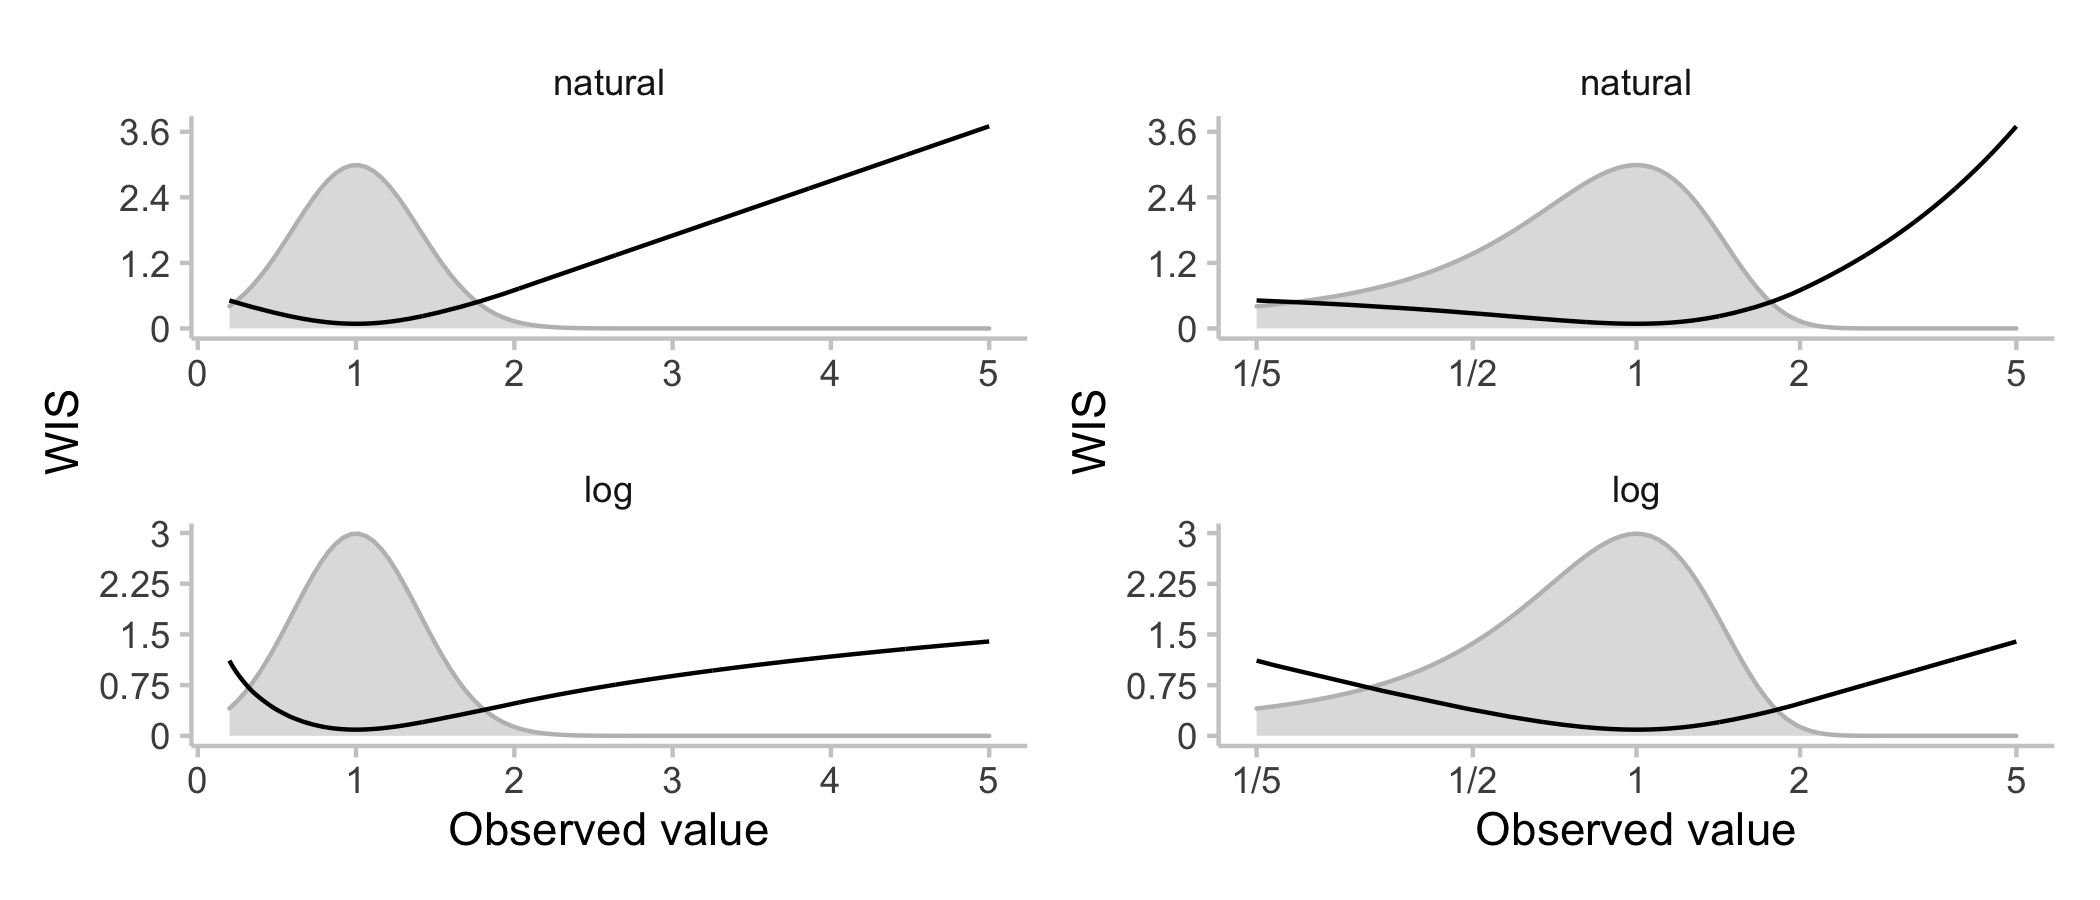
\includegraphics[width=0.99\textwidth]{output/figures/SIM-effect-log-score.png}
    \caption{Illustration of the weighted interval score on the natural and the log scale. The WIS
    (black line) is shown for a $\mathcal{N}(1, 0.2)$ predictive distribution (truncated at 0, density represented by the grey area) as a function of the observed value. 
    A: Scores computed on the natural scale (without prior transformation of the predictive distribution and the observed values). The x-axis is shown on a linear scale. C: Scores computed on the logarithmic scale (log-transforming the predictive distribution and the observed values prior to scoring). The x-axis is shown on a linear scale. B, D: Like A, C, but the x-axis is shown on a relative scale.} 
    \label{fig:change-in-scores}
\end{figure}


\section{Interpretation as scoring the exponential growth rate}
\label{sec:methods:growthrate}

Computing a score based on the logarithm of the forecast and the observation is also equivalent to scoring a forecast of the exponential growth rate of the forecast target. The exponential growth rate $r$ governs epidemic growth via (see e.g. \cite{wallingaHowGenerationIntervals2007})
%
\begin{linenomath*}
\begin{equation*}
y_{t + \Delta t} = y_t \cdot \exp(r \cdot \Delta t).
\end{equation*}
\end{linenomath*}
For small $\Delta t$ and $r$ this is approximately equivalent to
\begin{linenomath*}
\begin{equation*}
 y_{t + \Delta t} = y_t \cdot (1 + r \cdot \Delta t),
%y(t) \cdot \exp(r \cdot \Delta t) \approx y(t) \cdot (1 + r \cdot \Delta t),
\end{equation*}
\end{linenomath*}
%
which is sometimes used as an alternative definition ($r$ in this formulation is then called the multiplicative growth rate). Now assume that we predict one step time step ahead, i.e., at time $t$ we predict $y_{t + 1} = \hat{y}_{t + 1} + \varepsilon^*_{t+1}$. Moreover assume that $r$ is time-constant between $t$ and $t + 1$. The score is determined by the size of $\left|\varepsilon^*_{t+1}\right|$, the absolute error of the log-transformed incidence. 
%
\begin{linenomath*}
\begin{align*}
%\varepsilon^*_{t+1} & = \left|\log \hat{y}_{t + 1} - \log y_{t + 1} \right|\\
\varepsilon^*_{t+1} & = \log \hat{y}_{t + 1} - \log y_{t + 1} \\
& = \log \left[\exp(\hat{r}) \cdot y_t\right] - \log \left[\exp(r) \cdot y_t\right] \\
& = \hat{r} - r,
\end{align*}
\end{linenomath*}
where $\hat{r}$ is the predicted exponential growth rate as implied by $\hat{y}(t + 1)$. By log-transforming both the predicted value and the observation prior to applying the absolute error we thus just assess the error in the predicted exponential growth rate. If we apply the same reasoning to an $n$-week-ahead forecast and assume that the growth rate is piece-wise constant with value $r_t$ on $[t, t + 1)$, we get
%
\begin{linenomath*}
\begin{align*}
\epsilon^* & = \log \hat{y}_{t + n} - \log y_{t + n}\\
& = \log\left[\exp\left(\prod_{i = 0}^{n - 1}\hat{r}_{t + i}\right) \cdot y_t\right] - \log\left[\exp\left(\prod_{i = 0}^{n - 1}r_{t + i} \right) \cdot y_t\right]\\
& =   \prod_{i = 0}^{n - 1}\hat{r}_{t + i} \ - \ \prod_{i = 0}^{n - 1}r_{t + i}.
\end{align*}
\end{linenomath*}
We thus evaluate the error in the cumulative growth over the considered $n$-week period.

\subsection{Effects on model rankings}
\label{sec:methods:rankings}
Rankings between different forecasters based on their scores may change through the log-transformation both when looking at aggregate scores as well as when looking at a single forecast. As an example for the effect on a single forecast, consider two forecasters, A and B. Both issue a single 50\%-prediction interval for a target which later resolves as 1. Forecaster A issues the interval [0.5, 2], while forecaster B issues [0.9. 2.5]. On the natural scale, the score would equal the dispersion of the forecast, i.e. the length of this interval (since the observed value falls within the prediction interval). Forecaster A would receive a score of $2 - 0.5$ = 1.5, beating forecaster B who would receive a score of $2.5 - 0.9 = 1.6$. When we transform the forecast, forecaster A receives a score of $\log (\frac{2}{0.5}) = 1.39$, while forecaster B obtains a score of $\log (\frac{2.5}{0.9}) = 1.02$ and now wins over forecaster A. The main difference between forecaster A and B is that forecaster A has issued a prediction interval ([0.5, 2]) that was more symmetric around the true value than the interval issued by forecaster B ([0.9. 2.6], which was more skewed). This means that in relative terms, Forecaster B was noticeably closer to the true value with the lower bound of their prediction interval, while only being slightly further away with the upper interval. This implies that scores on the log scale may treat (one-sided) outlier forecasts more leniently. 

Overall model rankings would be expected to differ even more when scores are averaged across multiple forecasts or targets. The change in rankings of aggregate scores is not mainly driven by the kinds of changes in model rankings for single forecasts just discussed. Rather, as observations from exponential processes are likely to be on very different absolute scales, large observations will account for the majority of absolute score but will not dominate relative scores in the same way. Evaluating forecasts based on relative errors may help with comparing performance across different targets. However, log-transforming forecasts and observations may also result in the opposite extreme because small absolute errors (e.g. predicting 9, rather than 3 deaths) may be large in relative terms if the quantity to forecast is very small. This can be exacerbated when forecasts are restricted to discrete values, where relative steps between possible values become greater for values closer to zero. 

\begin{figure}[h!]
    \centering
    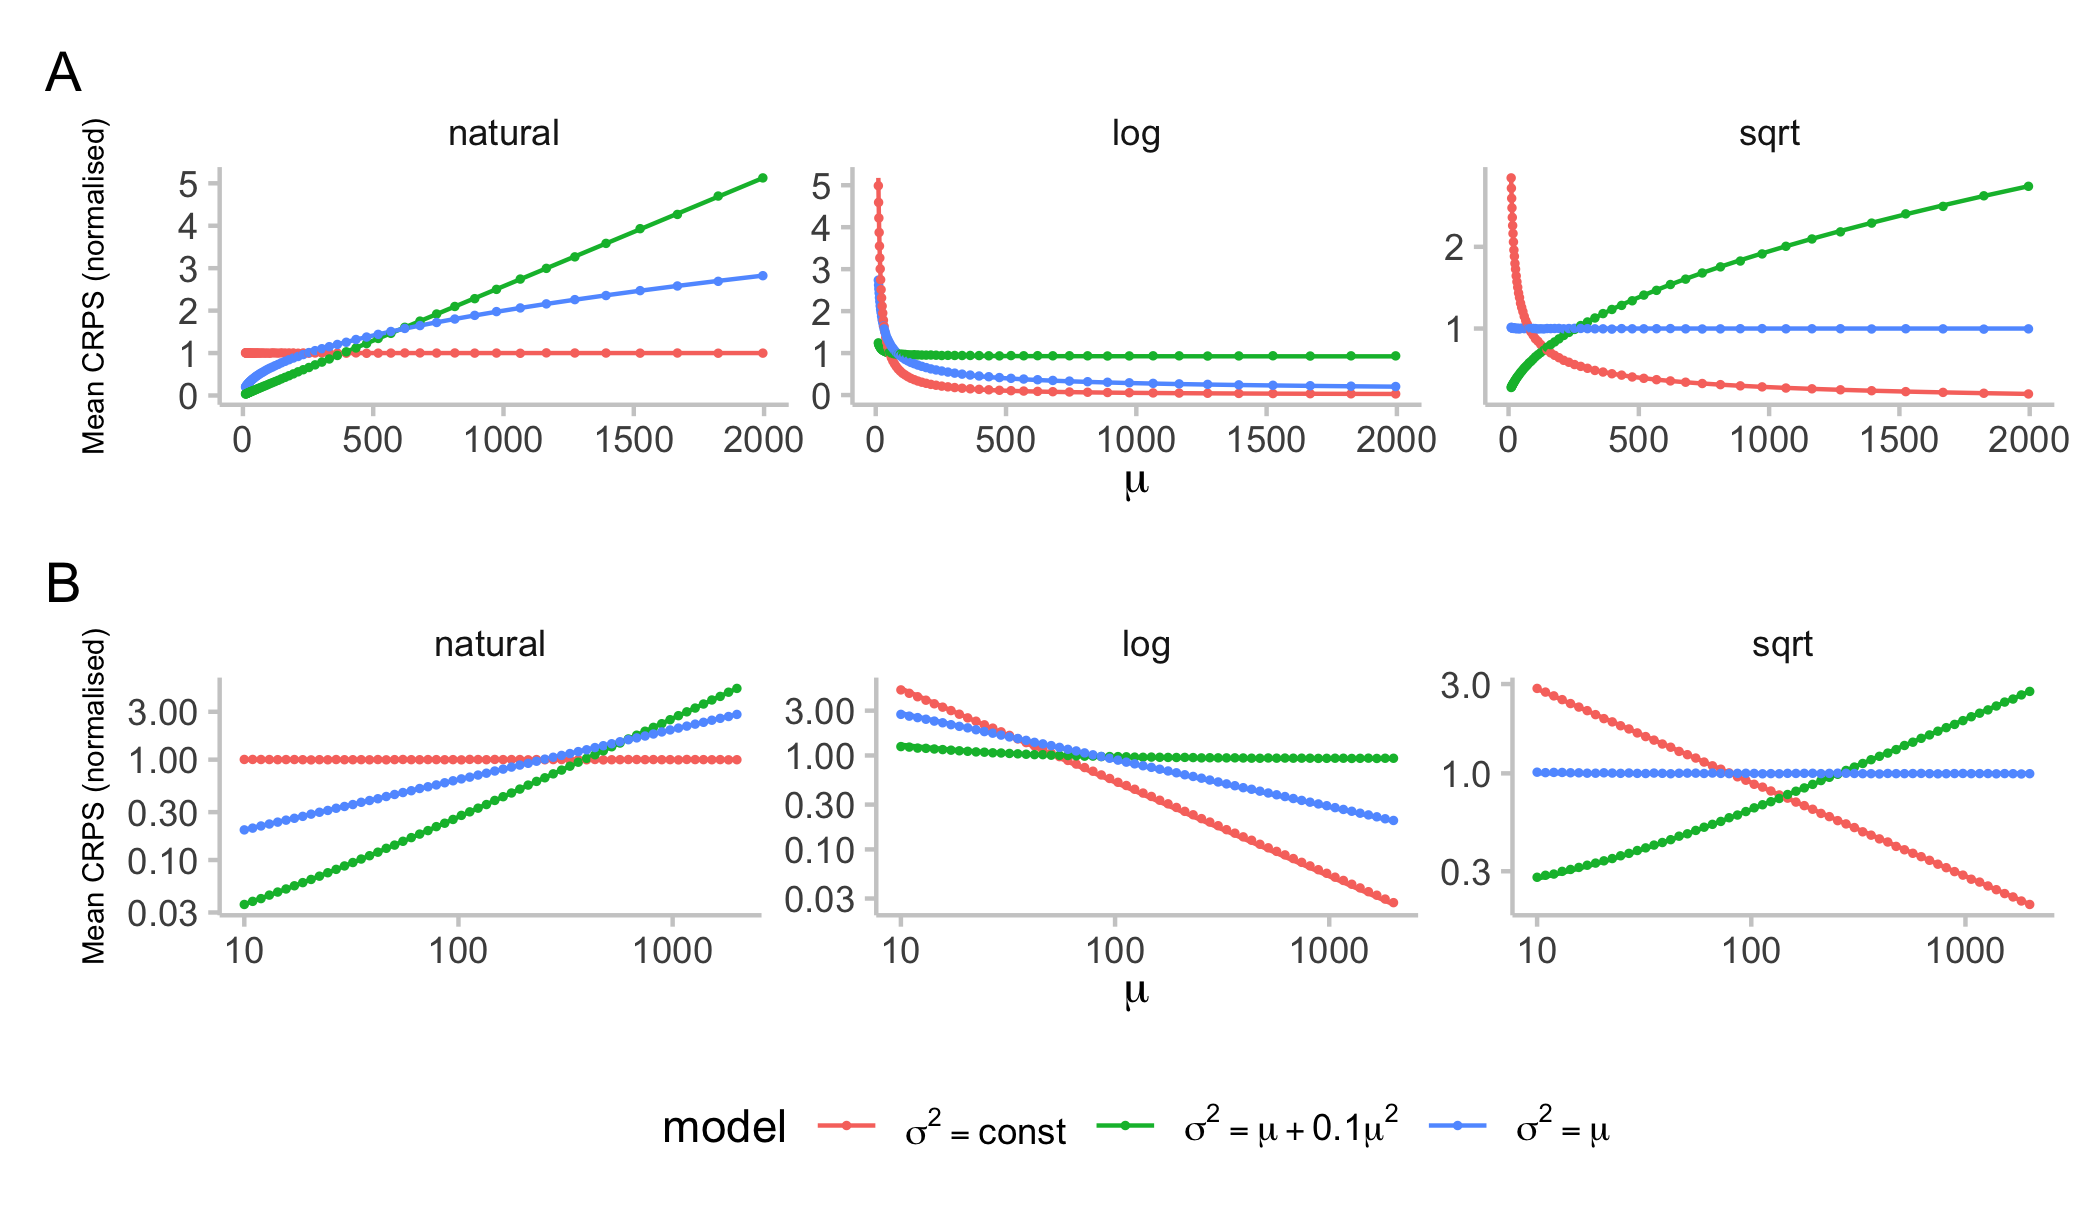
\includegraphics[width=0.99\textwidth]{output/figures/SIM-mean-state-size.png}
    \caption{Simulation showing how the relationship between mean and variance of the forecast quantity affects scores. 1,000 samples were drawn from different negative binomial distributions and scores were computed assuming an ideal forecaster (forecast distribution equal to data-generating distribution). Observations were simulated for different means of the negative-binomial distributions (representing, for example, the number of cases in differently sized states) as well as different relationships between mean and variance (representing, for example, three different infectious processes). The variance of the negative binomial is given as $\sigma^2 = \mu + \mu^2 / \theta$, meaning that for large theta the negative binomial distribution is equal to the Poisson distribution. We used values of $\theta = 0.1$ (red), 1 (green) and 1b (blue). To make the scores for the different distributions comparable, scores were normalised to one, meaning that the mean score for every distribution (red, green, blue) is one. 
    A: Normalised WIS for ideal forecasts with increasing means of three distribution with different relationships between mean and variance. B: A but with log scale axis.}
    \label{fig:SIM-wis-state-size-mean}
\end{figure}

Whether or not forecast targets with smaller quantities receive higher scores than those for targets with larger quantities, depends on the exact relationship between the mean and the variance of the quantity of interest. To provide a better intuition, we simulated count data following a negative binomial distribution. For these simulated data, log predictions for small quantities received on average higher scores than forecasts for large quantities if the mean and the variance grew at the same rate $\sigma^2 = \mu$, about equal scores when the variance grew at a rate of $\sigma^2 = \mu + \mu^2$, and smaller scores when the variance grew faster than that (Figure \ref{fig:SIM-wis-state-size-mean}). 

\subsection{Practical considerations}
\label{sec:methods:considerations}

The log-transformation (among many other transformations) is permissible (in the sense that it preserves propriety of the score), because it is a strictly monotonic transformation. Even though actual rankings between models may change, forecasters will in expectation still minimise their score if they report a predictive distribution that is equal to the data-generating distribution. The order of the operations matters, and applying a transformation after scores have been computed generally does not guarantee propriety. In the specific example, taking the logarithm of the scores, rather than scoring the log-transformed forecasts and data, results in an improper score. This is because taking the logarithm of the WIS / CRPS results in a score that does not penalise outliers enough and therefore incentivises overconfident predictions. We illustrate this point using simulated data in Figure \ref{fig:log-improper}, where it can easily be seen that overconfident models perform best in terms of the log WIS. 

\begin{figure}[h!]
    \centering
    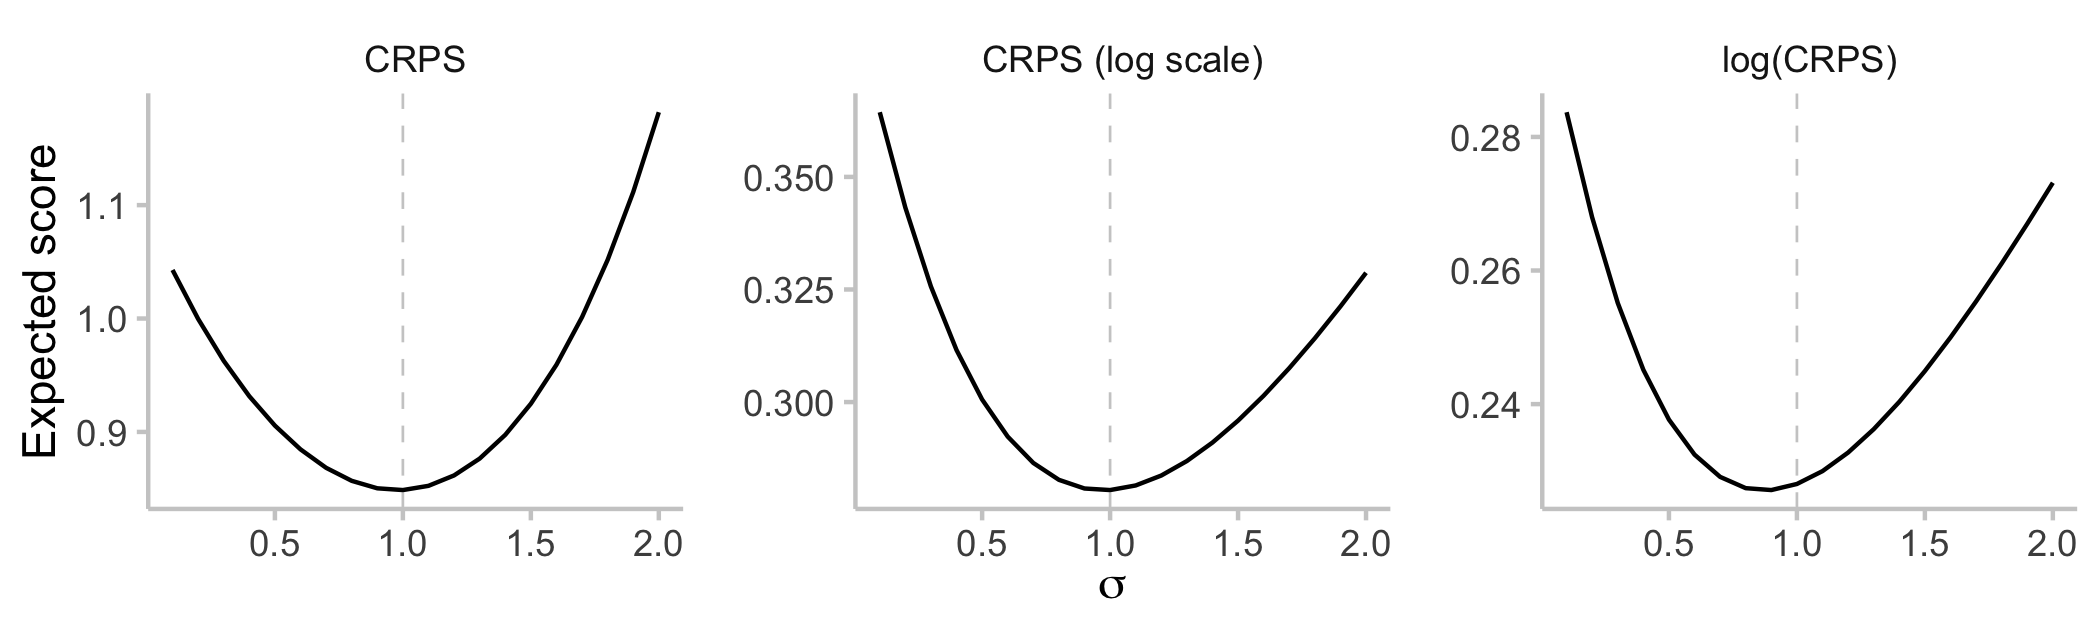
\includegraphics[width=0.99\textwidth]{output/figures/example-log-first.png}
    \caption{Scores for different forecasts evaluated using the WIS, the WIS on the log-scale and the logarithm of the WIS. We simulated 1000 observations $Y_i = {\rm e}^{x_i}$, with $x_i \text{ iid} \sim \mathcal{N}(0, 1)$. We then simulated 20 forecasters who would issue a predictive distribution $F = {\rm e}^{x_i}$, with $x \sim \mathcal{N}(0, \sigma)$, with values of $\sigma$ ranging from 0.1 to 2. For forecasts evaluated by the WIS and the WIS on log-transformed values, the score is minimised when the predictive distribution equals the data-generating distribution. When taking the logarithm of the WIS, scores are minimised for a predictive distribution that is too narrow compared to the data-generating distribution.}
    \label{fig:log-improper}
\end{figure}

In practice, one issue with the log-transformation is that it cannot readily be applied to negative numbers or zero values. In addition, it may be difficult to reliably evaluate relative errors when dealing with small discrete values. In an epidemiological setting that involves count data, negative values should likely be omitted entirely. One solution to deal with zeroes and small values is to also exclude those from ongoing analysis. An alternative is to add a small quantity, such as 1, to all observations and predictions before taking the logarithm as is common practice when log-transforming counts. This represents a strictly monotonic transformation and therefore preserves propriety of the resulting score. The choice of the number to add influences scores and rankings, as measures of relative errors shrink when adding a constant to the forecast and the observation. Adding something to the forecasts and observations changes scores for forecasts of small quantities most, as relative errors shrink more the smaller the original value before adding a constant. In principle, it would also be possible to exploit the difference in how scores are affected in order to equalise scores for forecasts of quantities across different scales by adding a larger number (e.g. 100 or 10,000) if average scores are dominated too strongly by forecasts for small quantities. 



\section{Empirical example: the European Forecast Hub}
\label{sec:results}

As an empirical example for evaluating forecasts on the natural and on the log scale we use forecasts from the European Forecast Hub \citep{europeancovid-19forecasthubEuropeanCovid19Forecast2021, sherrattPredictivePerformanceMultimodel2022}. 
The European COVID-19 Forecast Hub is one of several COVID-19 Forecast hubs (together with a Hub in the US \citep{cramerEvaluationIndividualEnsemble2021} and one in Germany and Poland \citep{bracherShorttermForecastingCOVID192021}) which have been systematically collecting, aggregating and evaluating forecasts of several COVID-19 targets created by different teams every week. Forecasts are made one to four weeks ahead into the future and follow a quantile-based format with a set of 22 quantiles plus the median ($0.01, 0.025, 0.05, ..., 0.5, ... 0.95, 0.975, 0.99$). 

The forecasts used for the purpose of this illustration are forecasts submitted between March 8 2021 and October 18 2021 for reported cases and deaths from COVID-19. We filtered all forecasts submitted to the Hub to only include models which have submitted forecasts for both deaths and cases for 4 horizons in 32 locations on at least 16 forecast dates (see Figure \ref{fig:HUB-num-avail-models}). Where not otherwise stated, we report results for a two-week-ahead forecast horizon. 

In addition to the WIS we use pairwise comparisons \citep{cramerEvaluationIndividualEnsemble2021} to evaluate the relative performance of models across countries in the presence of missingness. In a first step, score ratios are computed for all pairs of models by taking the set of overlapping forecasts between the two models and dividing the score of one model over the score achieved by the other model. The relative skill for a given model compared to others is then obtained by taking the geometric mean of all score ratios which involve that model. Low values are better, and the average model receives a relative skill score of 1. 

\begin{figure}[h!]
    \centering
    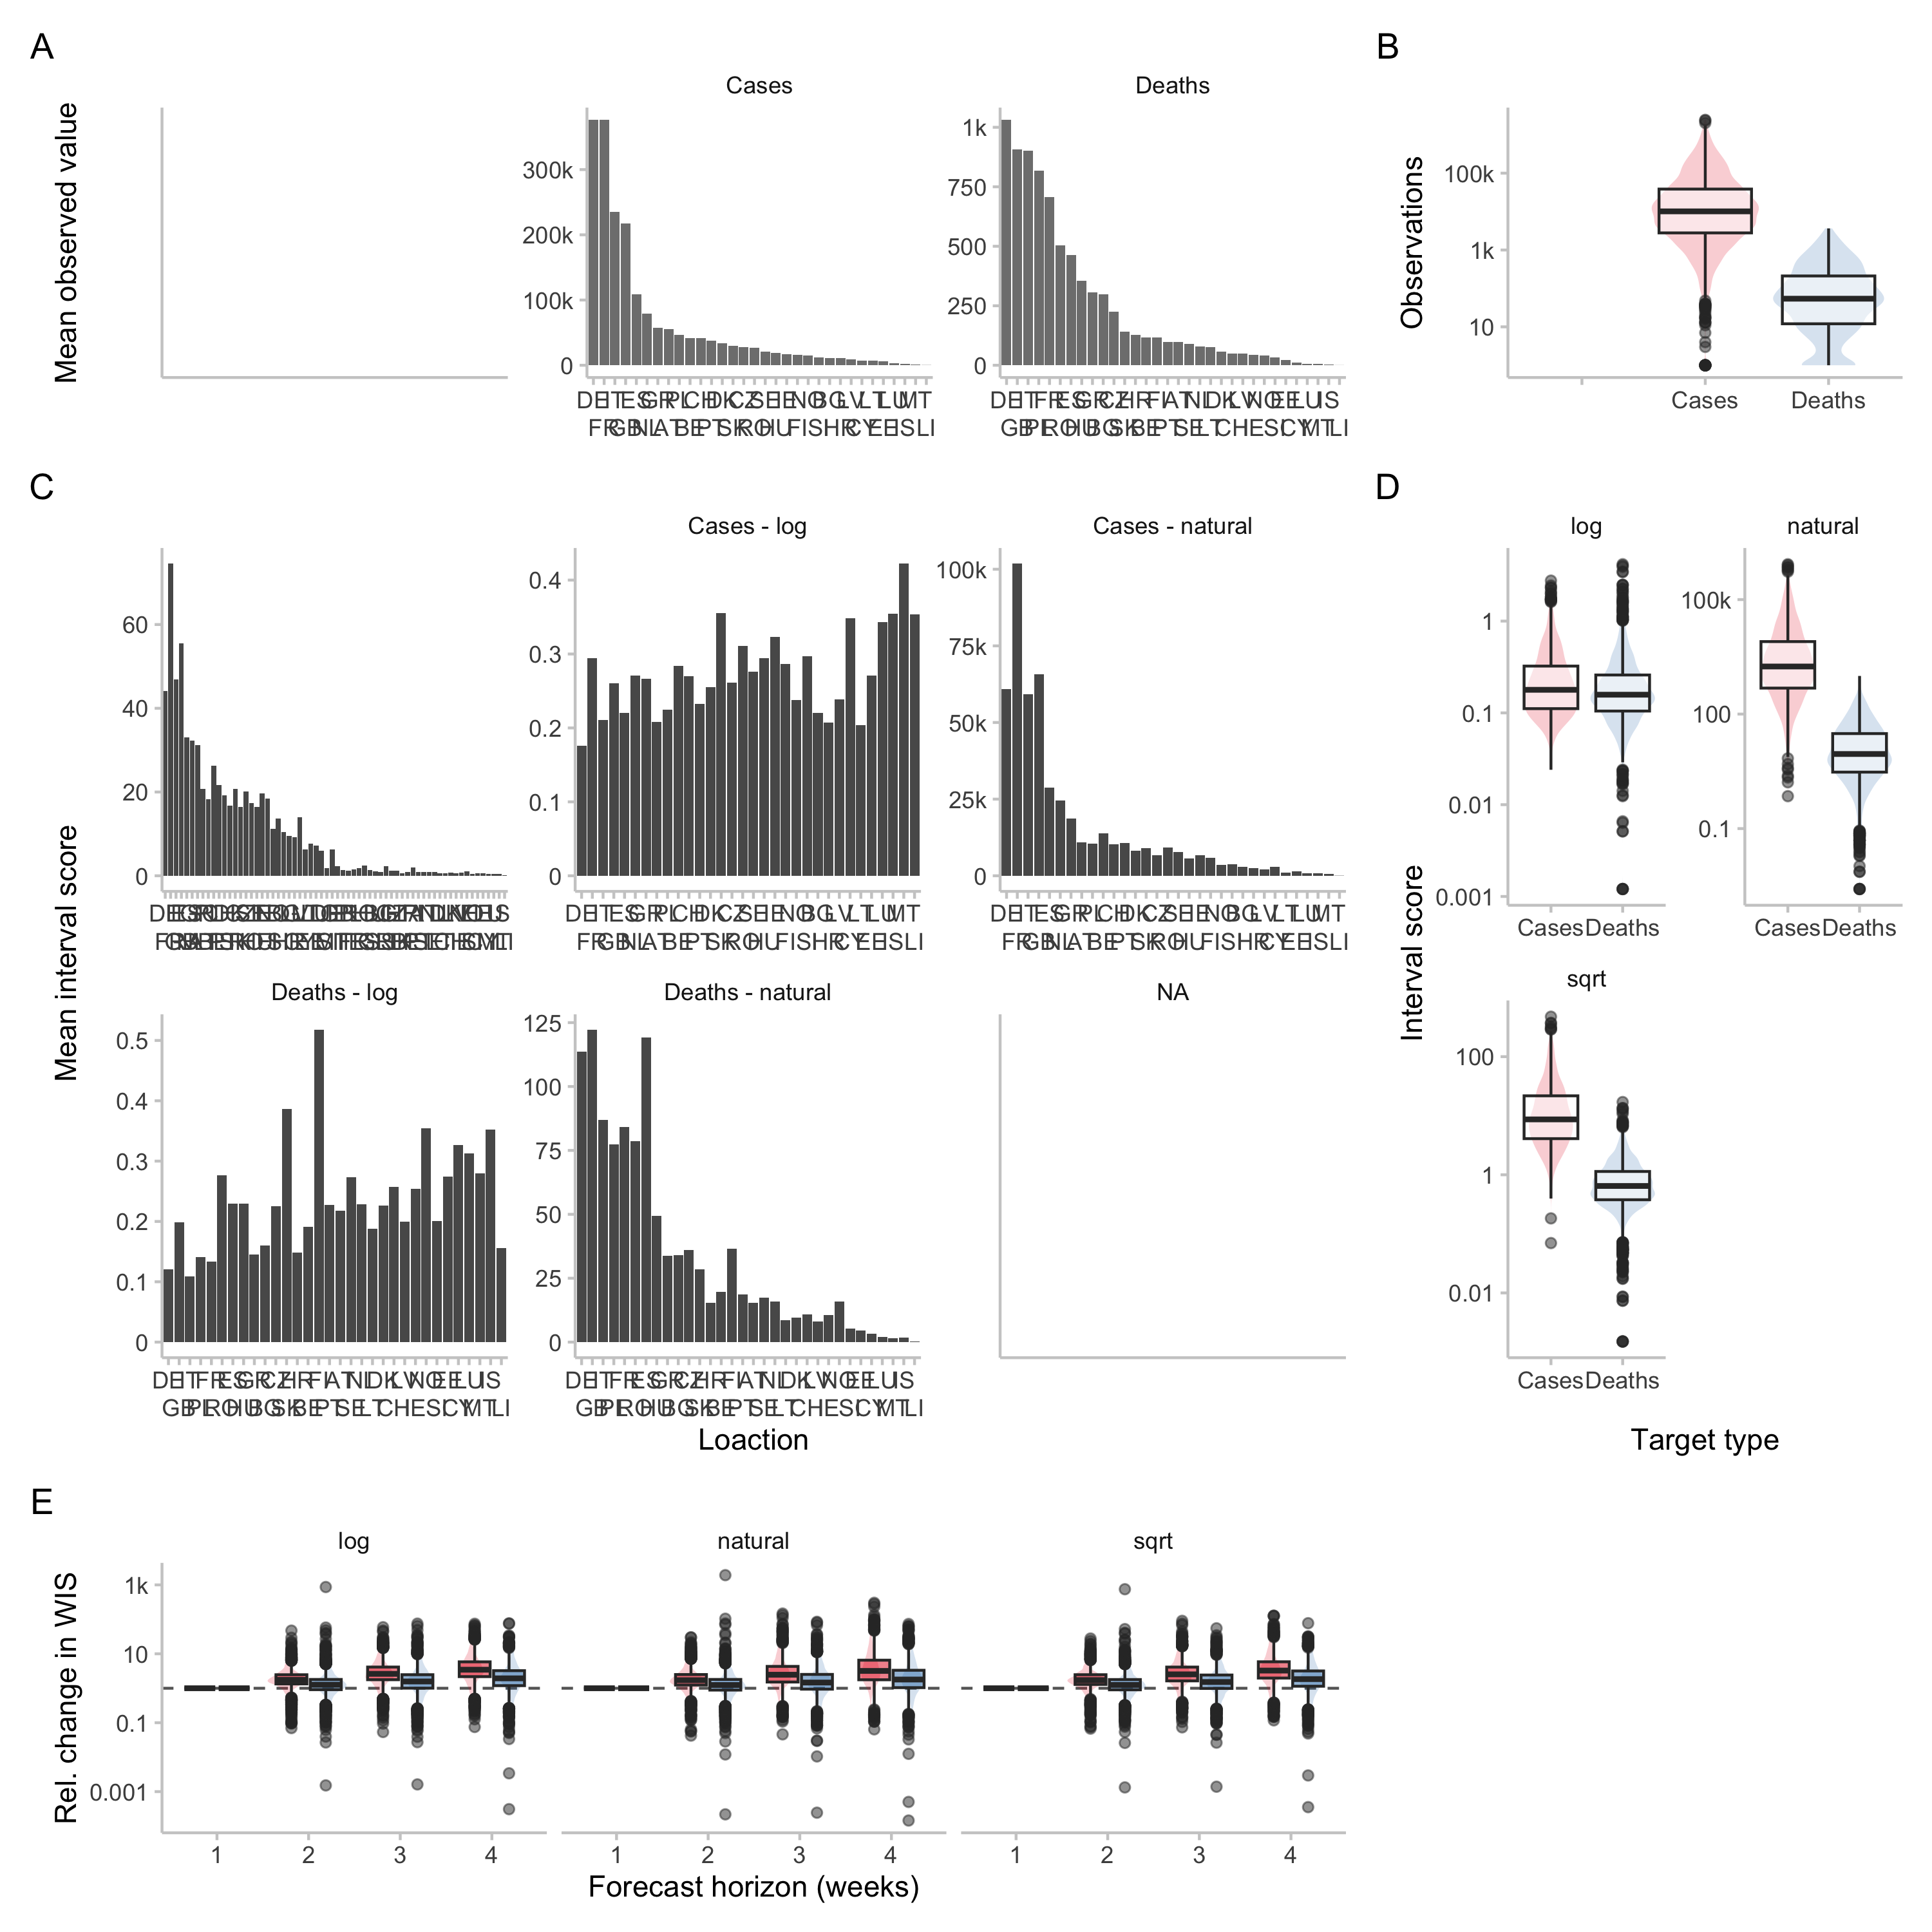
\includegraphics[width=0.99\textwidth]{output/figures/HUB-mean-obs-location.png}
    \caption{Observations and scores across locations and forecast horizons for the European COVID-19 Forecast Hub data. Locations are sorted according to the mean observed value in that location. 
    A: Average (across all time points) of observed cases and deaths for different locations. B: Corresponding boxplot (y-axis on log-scale) of all cases and deaths. C: Scores for two-week-ahead forecasts from the EuroCOVIDhub-ensemble (averaged across all forecast dates) for different locations, evaluated on the natural as well as the logarithmic scale. D: Corresponding boxplots of all individual scores for two-week-ahead predictions. E: Boxplots for the relative change of scores for the EuroCOVIDhub-ensemble across forecast horizons. For any given forecast date and location, forecasts were made for four different forecast horizons, resulting in four scores. All scores were divided by the score for forecast horizon one.}
    \label{fig:HUB-mean-locations}
\end{figure}

Across the dataset, the average number of observed cases and deaths varied considerably by location and target type (see Figure \ref{fig:HUB-mean-locations}A and B). On the natural scale, scores also varied considerably across targets (see Figure\ref{fig:HUB-mean-locations}D) and locations (see Figure\ref{fig:HUB-mean-locations}C). On the log scale, scores were more evenly distributed between targets (see Figure\ref{fig:HUB-mean-locations}D) and locations (see Figure\ref{fig:HUB-mean-locations}C). Both on the natural scale as well to a slightly lesser extent on the log scale, scores increased considerably with increasing forecast horizon (see Figure \ref{fig:HUB-mean-locations}E). We hypothesise that this increase in scores across horizons represents the relative difficulty to forecast values into the future, which was noticeable both on the natural as well as the logarithmic scale. 

\begin{figure}[h!]
    \centering
    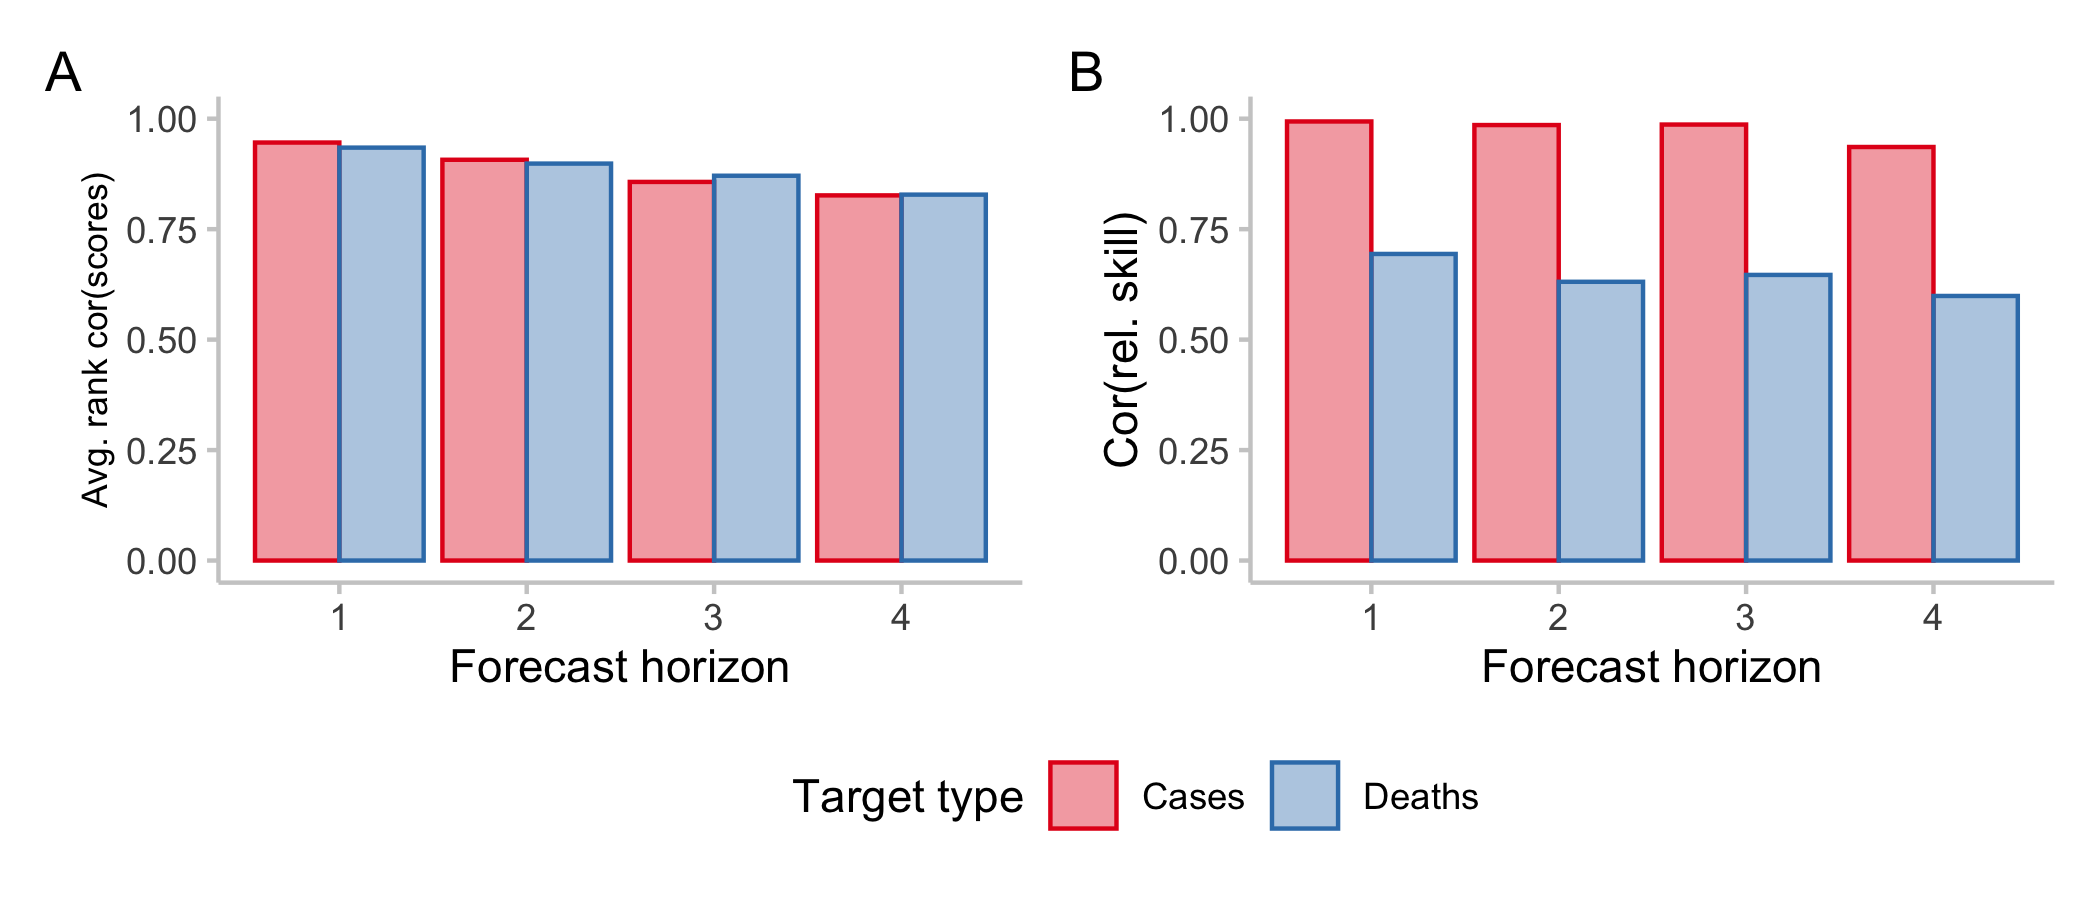
\includegraphics[width=0.99\textwidth]{output/figures/HUB-correlations.png}
    \caption{Correlations between observations and scores. A: Mean WIS for two-week-ahead predictions of the EuroCOVIDhub-ensemble against the average number of observations in a location. B: Average Spearman rank correlation of scores for individual forecasts from all models. For every individual target (defined by a combination of forecast date, target type, horizon, location), one score was obtained per model. Then, the rank correlation was computed between the scores for all models on the natural scale vs. on the log scale. All rank correlations were averaged and stratified by horizon and target type. C: Correlation between relative skill scores. For every forecast horizon and target type, a separate rel. skill score was computed per model using pairwise comparisons. The plot shows the correlation between the rel. skill scores on the natural vs. on the log scale.}
    \label{fig:HUB-cors}
\end{figure}

As expected on the natural scale, scores correlate strongly with the average number of observed cases and deaths (Spearman rank correlation: 0.96 and 0.97) in a given country (see Figure\ref{fig:HUB-mean-locations}A, B). We report the Spearman rank correlation here, rather than the Pearson correlation, so that correlations remain the same regardless of whether we look at observed values on the log or natural scale. 
On the log scale, the correlation is much weaker and slightly negative, at least in terms of rank correlation (Spearman correlation: -0.33 and -0.36), implying a tendency towards larger scores in countries with lower mean incidences. 


\begin{figure}[h!]
    \centering
    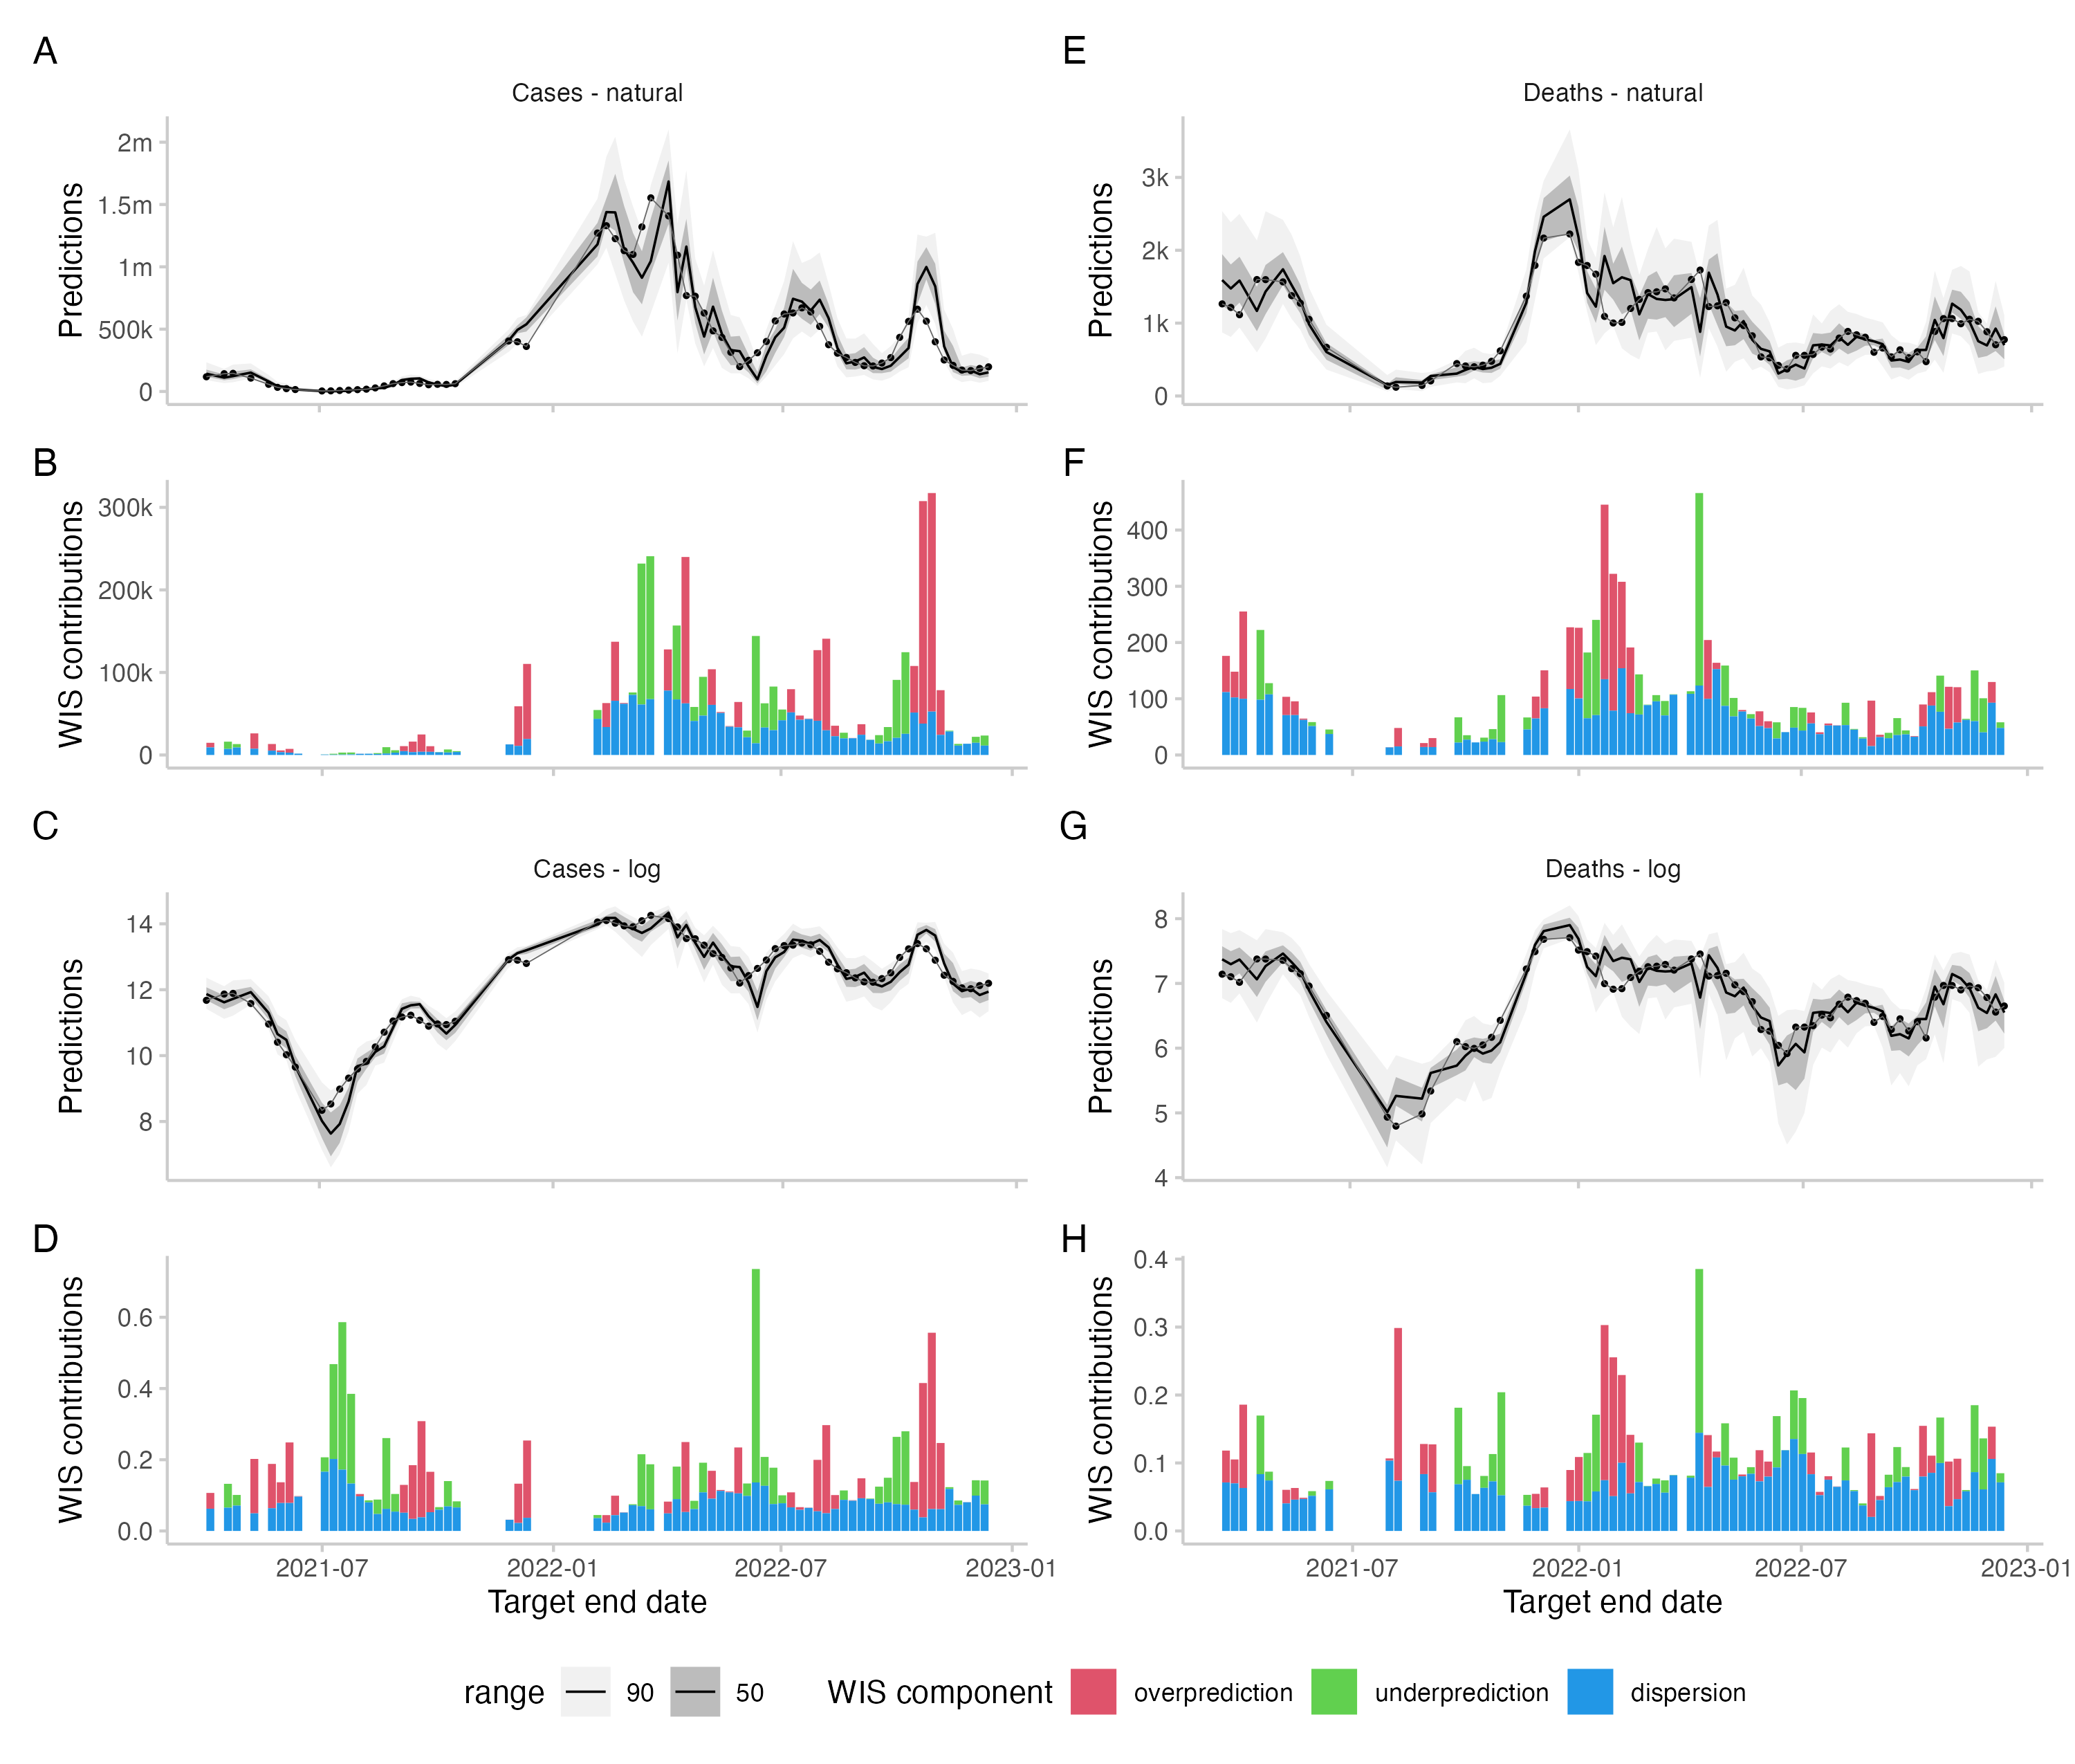
\includegraphics[width=0.99\textwidth]{output/figures/HUB-model-comparison-ensemble.png}
    \caption{
    Forecasts and scores for two-week-ahead predictions from the EuroCOVIDhub-ensemble made in Germany. A, E: 50\% and 90\% prediction intervals and observed values for cases and deaths on the natural scale. B, F: Corresponding scores. C, G: Forecasts and observations on the log scale. D, H: Corresponding scores. 
    }
    \label{fig:HUB-model-comparison-ensemble}
\end{figure}


For \textit{individual} forecasts, rankings between models for single forecasts are mostly preserved, with differences increasing across forecast horizons (see Figure \ref{fig:HUB-cors}B). When evaluating performance \textit{averaged across} different forecasts and forecast targets, relative skill scores of the models change considerably. The change is stronger for cases than for deaths (Figure \ref{fig:HUB-cors}C) and possibly tends to increase with increasing forecast horizon. 

When comparing examples of forecasts on the natural scale with those on the log scale (see Figures \ref{fig:HUB-model-comparison-ensemble}, \ref{fig:HUB-model-comparison-baseline}, \ref{fig:HUB-model-comparison-epinow}) a few interesting patterns emerge. Missing the peak, i.e. predicting increasing numbers while actual observations are already falling, tends to contribute a lot to overall scores on the natural scale (see forecasts in May in Figure \ref{fig:HUB-model-comparison-ensemble}A, B). On the log scale, these have less of an influence, as errors are smaller in relative terms (see \ref{fig:HUB-model-comparison-ensemble}C, D). We hypothesise that the lower correlation between skill scores for cases (compared to the correlation of scores for deaths) as displayed in Figure \ref{fig:HUB-cors}C is related to the fact that outlier forecasts missing the peak are more common for cases than for deaths, and therefore relative skill scores are more strongly affected for cases. 
Conversely, failure to predict an upswing while numbers are still low, is less severely punished on the natural scale (see forecasts in July in Figure \ref{fig:HUB-model-comparison-ensemble} A, B), as overall absolute errors are low. On the log scale, missing lower inflection points tends to lead to more severe penalties (see Figure \ref{fig:HUB-model-comparison-ensemble}C, D)). One can also observe that on the natural scale, scores tend to track the overall level of the target quantity (compare for example forecasts for March-July with forecasts for September-October in Figure \ref{fig:HUB-model-comparison-ensemble}E, F). On the log scale, scores do not exhibit this behaviour and rather increase whenever forecasts are far away from the truth in relative terms, regardless of the overall level of observations. 

\begin{figure}[h!]
    \centering
    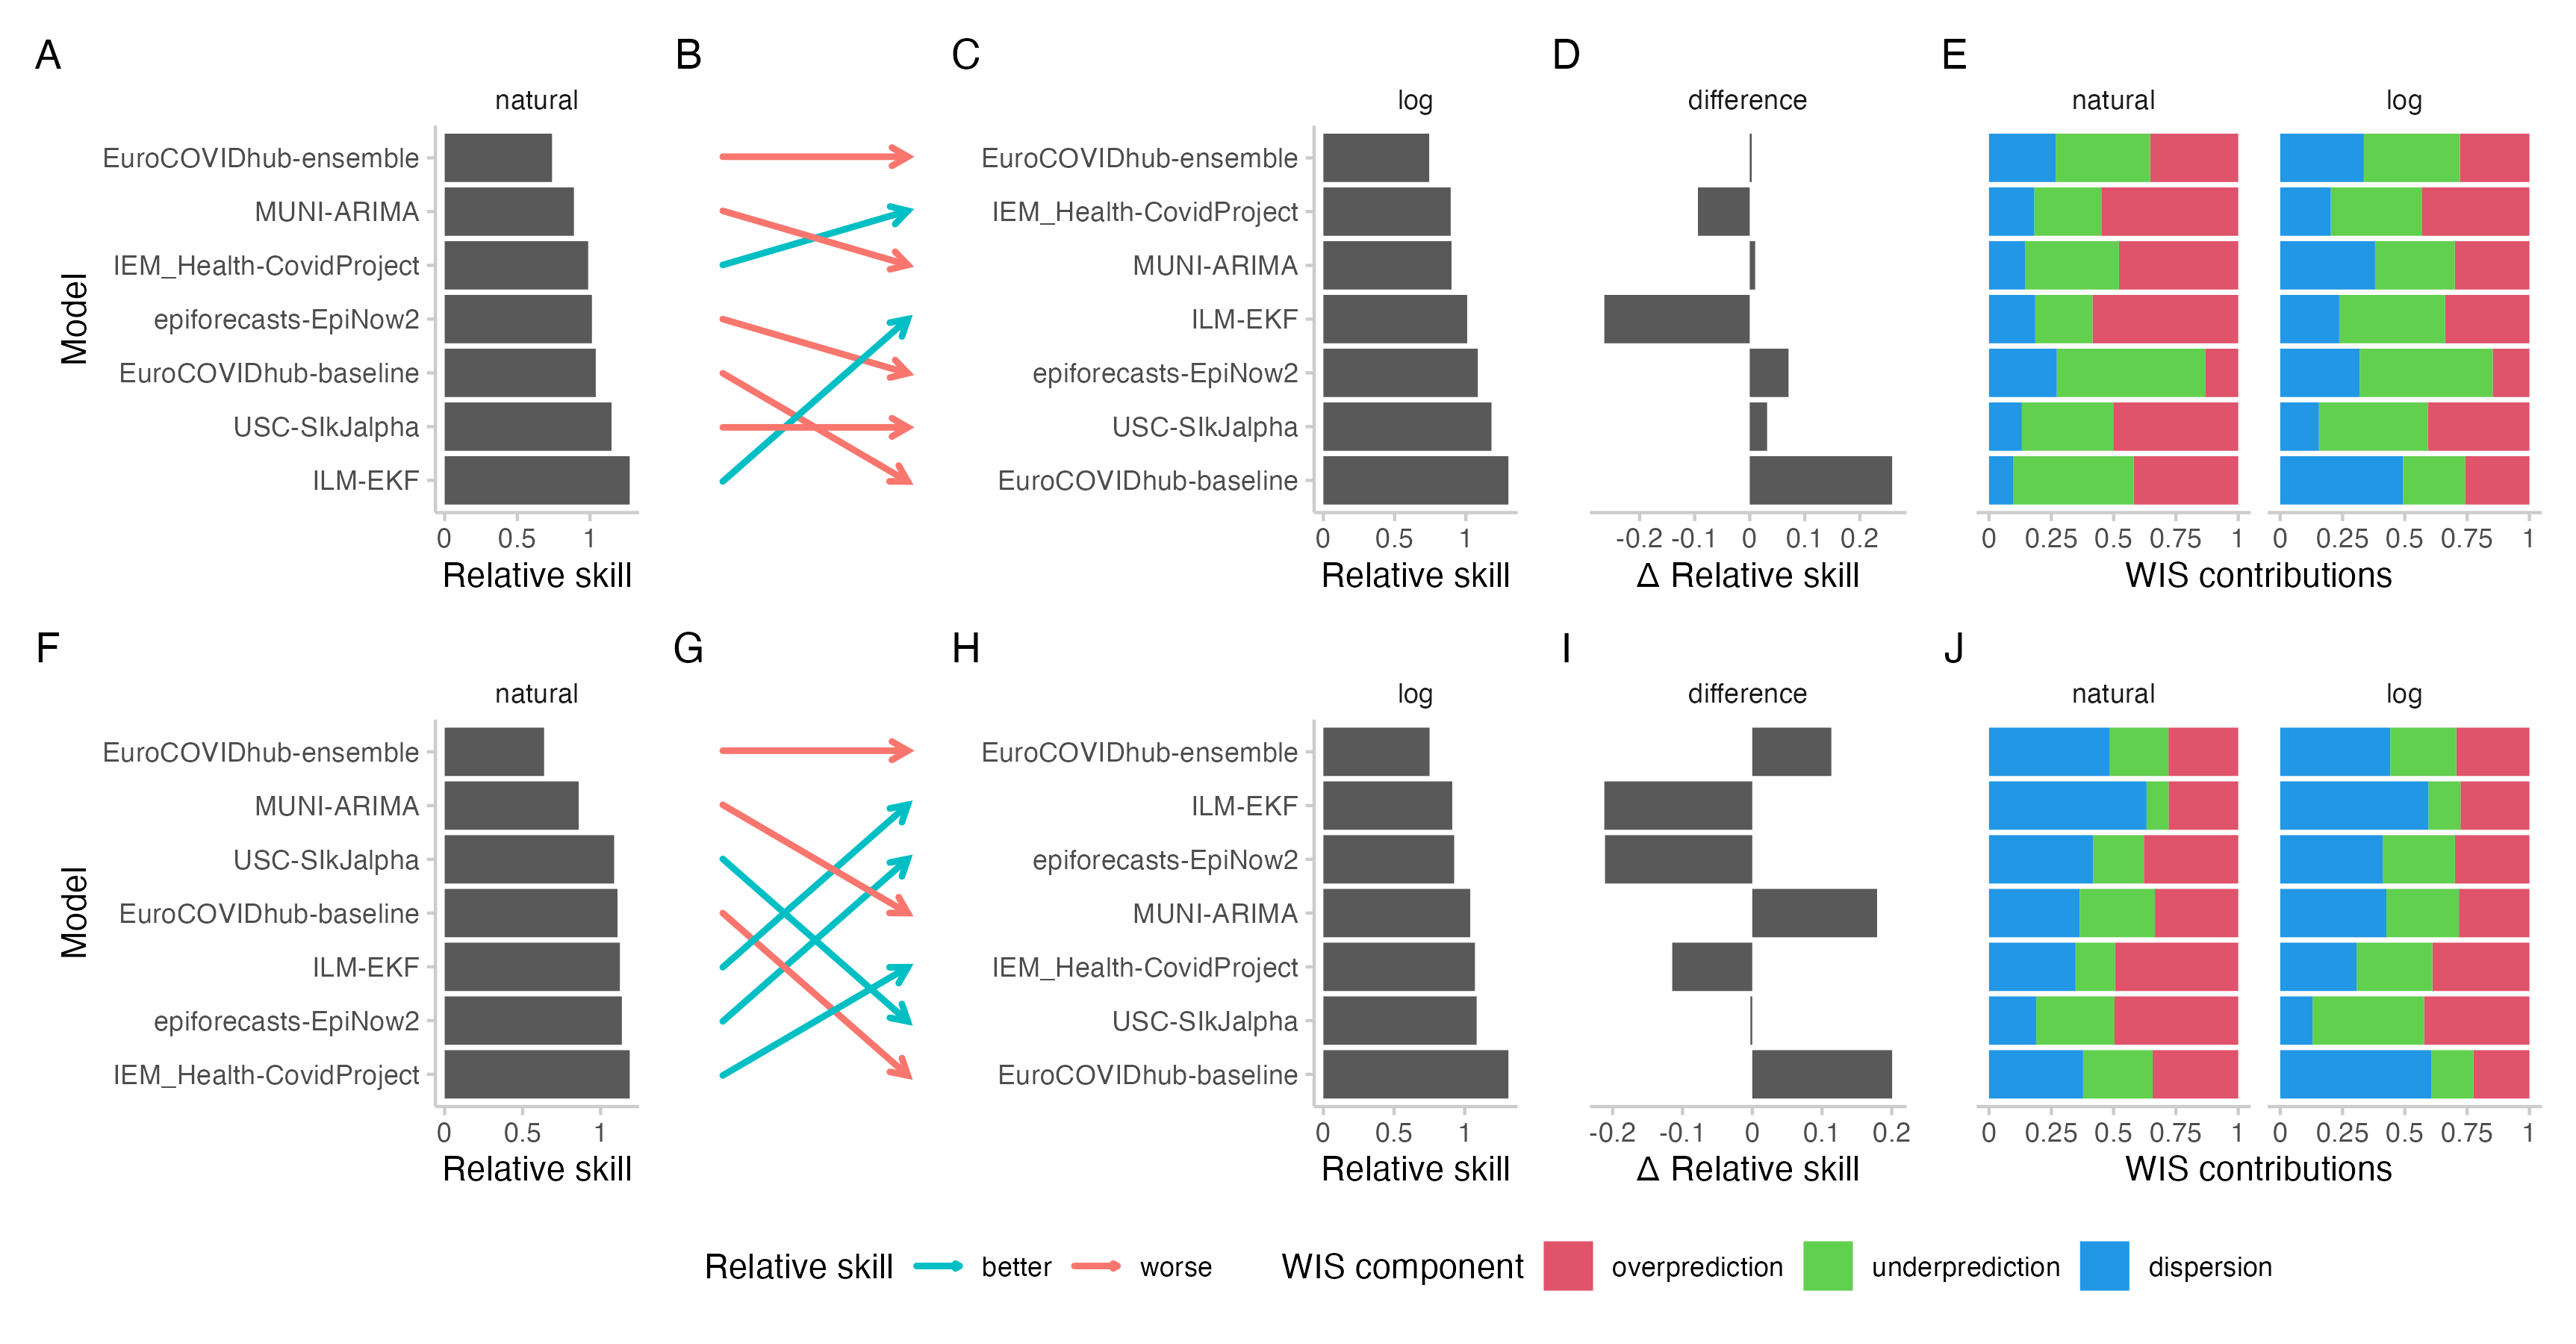
\includegraphics[width=0.99\textwidth]{output/figures/HUB-pairwise-comparisons.png}
    \caption{Changes in model ratings as measured by relative skill for two-week-ahead predictions for cases (top row) and deaths (bottom row). A: Relative skill scores for case forecasts from different models submitted to the European COVID-19 Forecast Hub computed on the natural scale. B: Change in rankings as determined by relative skill scores when moving from an evaluation on the natural scale to one on the logarithmic scale. C: Relative skill scores based on scores on the log scale. D: Difference in relative skill scores computed on the natural and on the logarithmic scale. E: Relative contributions of the different WIS components (overprediction, underprediction, and dispersion) to overall model scores on the natural and the logarithmic scale. F, G, H, I, J, K: Analogously for deaths.}
    \label{fig:HUB-rank-order}
\end{figure}


The rank order of different forecasting models (see Figure \ref{fig:HUB-rank-order} indicates that models that do not make use of a exponential error model and thus would be biased towards under-prediction during periods of exponential growth, such as the MUNI-ARMA model, were ranked lower when using a log-transform. The epiforecasts-EpiNow2 forecast model, on the other hand~(created by co-authors of this study), which makes forecasts based on the behaviour of the reproduction number and thus implicitly uses an exponential error model, was the most impacted by the change to log-scale scoring moving from last place for reported cases to 4th place. Other models that are based on modelling the growth rate, such as the LANL-GrowthRate forecaster, do less well after a log-transform, indicating that this potential association between model structure and score under different approximations does not hold strictly. Encouragingly for the European Forecast Hub, the Hub ensemble, which is the forecast the organisers suggest forecast consumers make use of, remains one of the top forecasts across scoring schemes and indeed ranks higher for reported cases when a log-transform is used.

\section{Discussion}
\label{sec:discussion}

In this paper we proposed a log-transformation of forecasts and observed values prior to evaluation with the WIS (or CRPS) in order to address issues that arise when evaluating epidemiological forecasts based on a measure of absolute error. We gave a mathematical intuition for the transformation and showed that scores on the log scale can be interpreted as a) a measure of relative (multiplicative) prediction errors, as well as b) a score for a forecast of the exponential growth rate of the target quantity. 
When applying this approach to forecasts from the European COVID-19 Forecast Hub, we found overall scores on the log scale to be more equal across, time, location and target type (cases, deaths) than scores on the natural scale. Scores on the log scale were much less influenced by the overall incidence level in a country, and showed a slight tendency to be higher in locations with very low incidences. We found that model rankings changed noticeably, favouring models like epiforecasts-EpiNow2 which explicitly has an exponential error structure, and disfavouring models like MUNI-ARIMA which is a purely statistical model with a linear error structure. On the natural scale, missing the peak and overshooting was more severely penalised than missing the nadir and a following upswing in numbers. Both failure modes tended to be more equally penalised on the log scale (with undershooting receiving slightly higher penalties in our example). 

Applying a log-transformation prior to the WIS means that forecasts are evaluated in terms of relative errors and errors on the multiplicative growth rate, rather than absolute errors. The most important strength of this approach is that the evaluation better accommodates the exponential nature of epidemiological process and the types of errors forecasters who accurately model those processes are expected to make. The log-transformation also helps avoid issues with scores being strongly influenced by the order of magnitude of the forecast quantity, which can be an issue when evaluating forecasts on the natural scale. 
A potential downside is that forecast evaluation is unreliable in situations where observed values are zero or very small. Including very small values in prediction intervals (see e.g. Figure \ref{fig:HUB-model-comparison-baseline}) can lead to excessive dispersion values on the log scale. 
Similarly, locations with lower incidences may get disproportionate weight (i.e. high scores) when evaluating forecasts on the log scale. \cite{bracherEvaluatingEpidemicForecasts2021} argue that the large weight given to forecasts for locations with high incidences is a desirable property, as it reflects performance on the targets we should care about most. On the other hand, scoring forecasts on the log scale may be less influenced by outliers and better reflect consistent performance across time, space, and forecast targets. It also gives higher weight to another type of situation one may care about, namely one in which numbers start to rise from a previously low level. 
If one is interested in scoring a forecast of the multiplicative, rather than the exponential  growth rate, it may be better to use a different transformation, e.g. dividing every forecast and corresponding observed value by the previously last observed value when the forecast was made. 

The log-transformation is only one of many transformation that may be useful and appropriate in an epidemiological context. One easy transformation is to divide all forecasts by the population in a location, in order to obtain forecasts of standardised incidences per e.g. 100,000 inhabitants. A second transformation was mentioned above, namely converting forecasts into forecasts for the multiplicative growth rate by dividing numbers by the last observed value. One could also think about applying a Box-Cox or a square-root transformation in order to stabilise the variance of the forecasts. Another promising transformation would be to divide each forecast by the forecast of the previous week (and observations by the observation of the previous week), in order to obtain forecasts for week-to-week multiplicative growth rates, or alternatively, to ask forecasters to provide estimates of the weekly relative change applied to the latest data and subsequent forecast points directly. This would be akin to evaluating the shape of the predicted trajectory against the shape of the observed trajectory \citep[for a different approach to evaluation the shape of a forecast, see][]{srivastavaShapebasedEvaluationEpidemic2022}. This, unfortunately is not well defined in the context of forecasts stored as predictive quantiles, as the growth rate of the $\alpha$-quantile may be different from the $\alpha$-quantile of the growth-rate, but may be an interesting approach if predictive samples are available. What makes this approach of transforming forecasts before scoring particularly interesting is the possibility to construct composite scores as a weighted sum of scores based on different transformations. This would allow forecast consumers to assign explicit weights to different qualities of the forecasts they might care about. 

Exploring these different transformations is a promising avenue for future work that could help bridge the gap between modellers and policy makers by providing scoring rules that better reflect what forecast consumers actually care about. We have showed that the log-transformation can lead to significant changes in the relative rankings of models against each other, with potentially important implications for decision makers who rely on the knowledge of past performance to make a decision about which forecasts should inform future decisions. While it is commonly accepted that multiple proper scoring rules should usually be considered when comparing forecasts, we think this should be supplemented by considering different transformations of the data to obtain a richer picture of model performance. While we have produced this work as an initial case study, more work needs to be done to better understand the effects of applying a logarithmic or other transformations more comprehensively and in different contexts, and how it might affect decision making. 

\newpage

\appendix
\section{Supplementary information}

\begin{table}[h!]
    \centering
    
   \begin{tabular}{lllcc}
        \toprule
        target\_type & quantity & measure & natural & log\\
        \midrule
        Cases & Observations & mean & 19941 & 8.33\\
        Cases & Observations & sd & 43149 & 2.09\\
        Cases & Observations & var & 1861850319 & 4.35\\
        Deaths & Observations & mean & 222 & 3.65\\
        Deaths & Observations & sd & 481 & 2.07\\
        Deaths & Observations & var & 231025 & 4.29\\
        \addlinespace
        \hline
        \addlinespace
        Cases & WIS & mean & 4544 & 0.28\\
        Cases & WIS & sd & 17585 & 0.49\\
        Deaths & WIS & mean & 28 & 0.22\\
        Deaths & WIS & sd & 67 & 0.26\\
        \bottomrule
        \end{tabular}
    \caption{Summary statistics for observations and scores for forecasts from the ECDC data set.}
    \label{tab:HUB-summary}
\end{table}

\begin{figure}[h!]
    \centering
    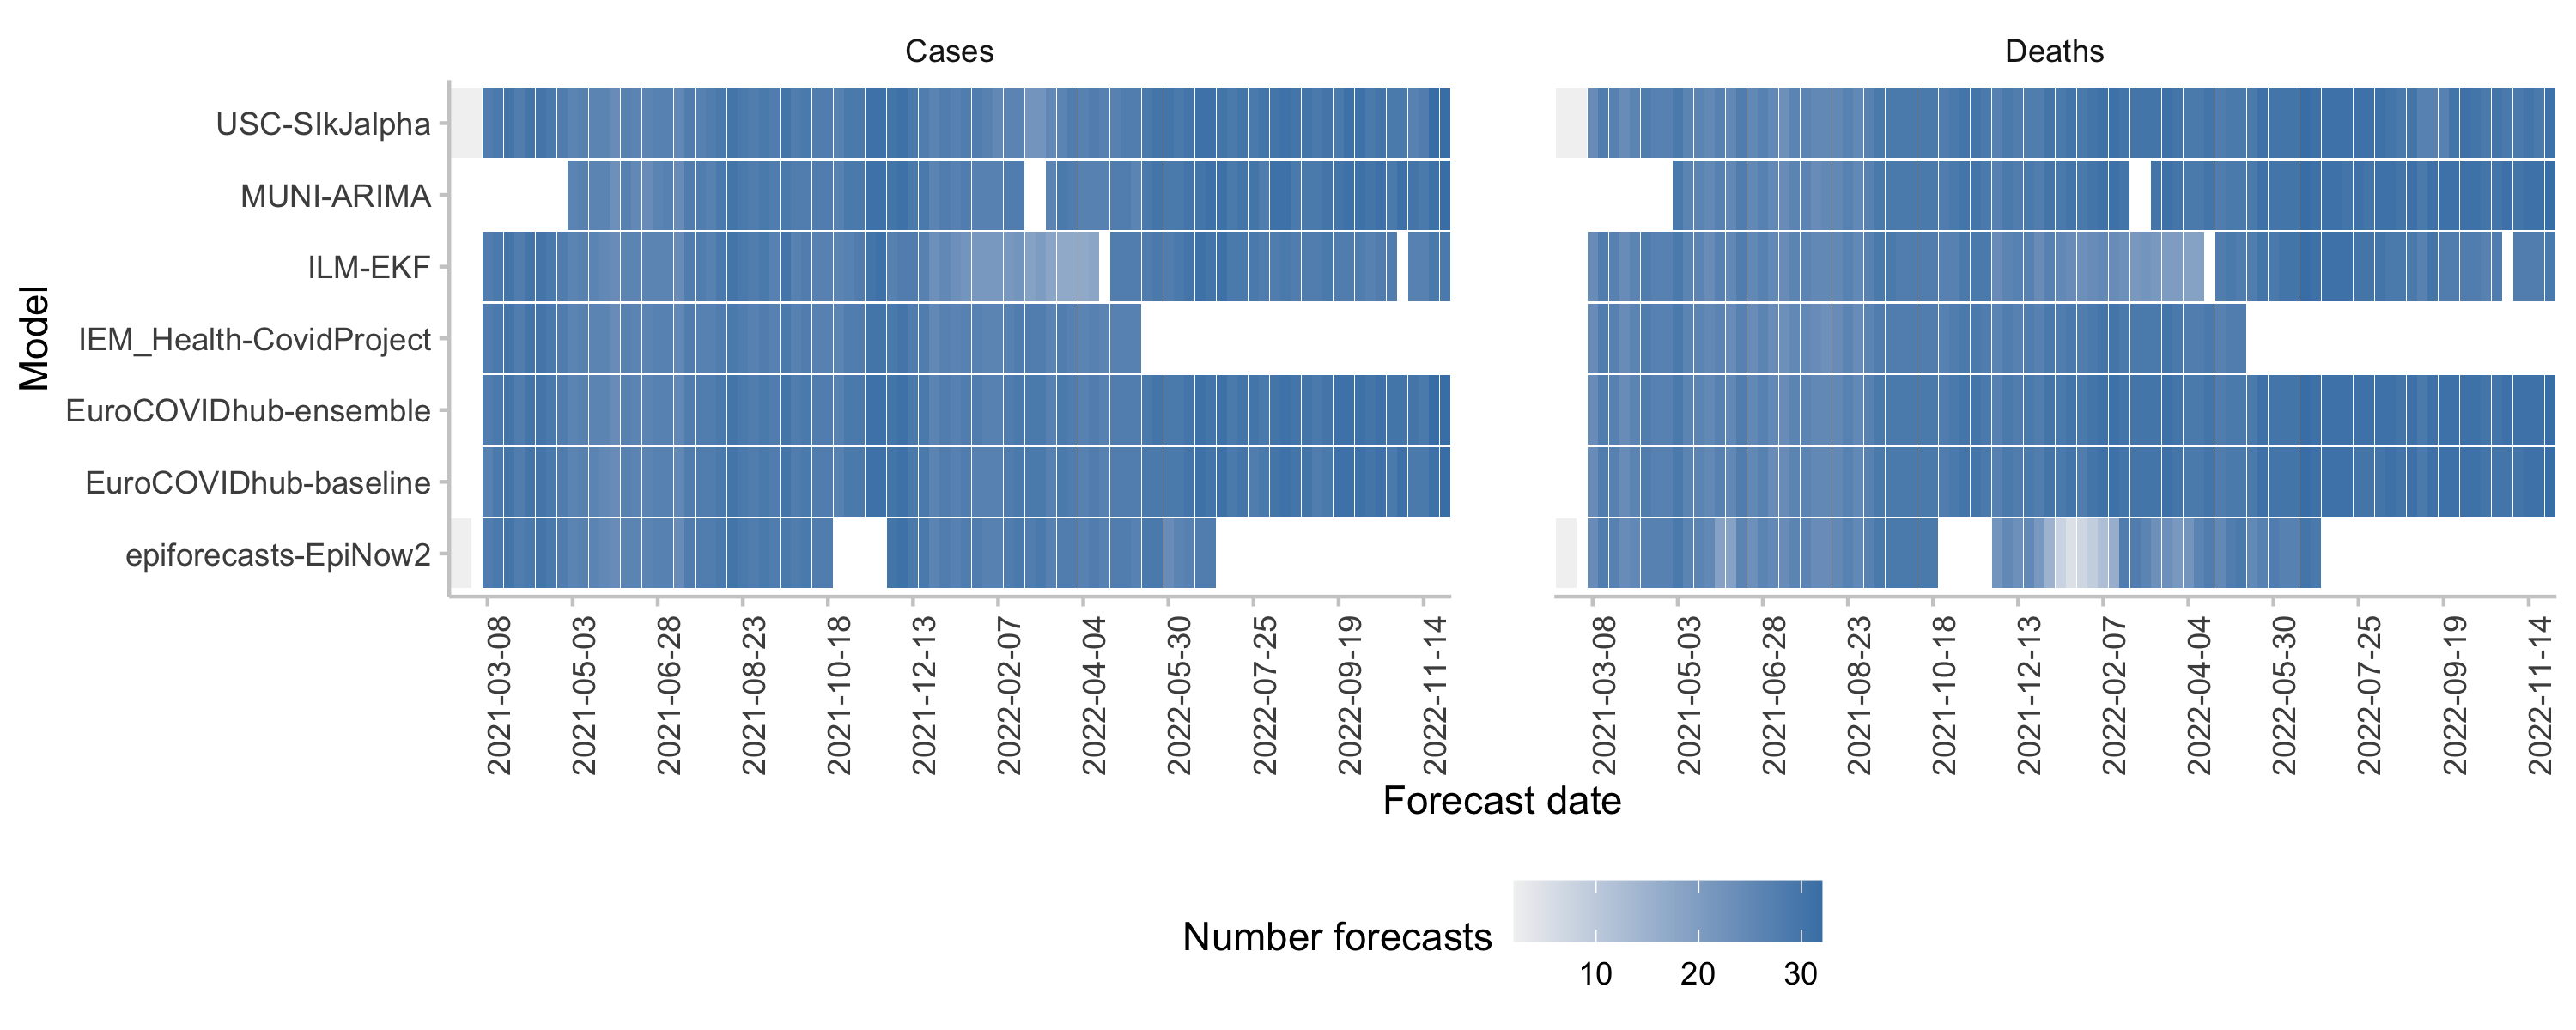
\includegraphics[width=0.99\textwidth]{output/figures/number-avail-forecasts.png}
    \caption{
    Number of forecasts available from different models for each forecast date. 
    }
    \label{fig:HUB-num-avail-models}
\end{figure}


\begin{figure}[h!]
    \centering
    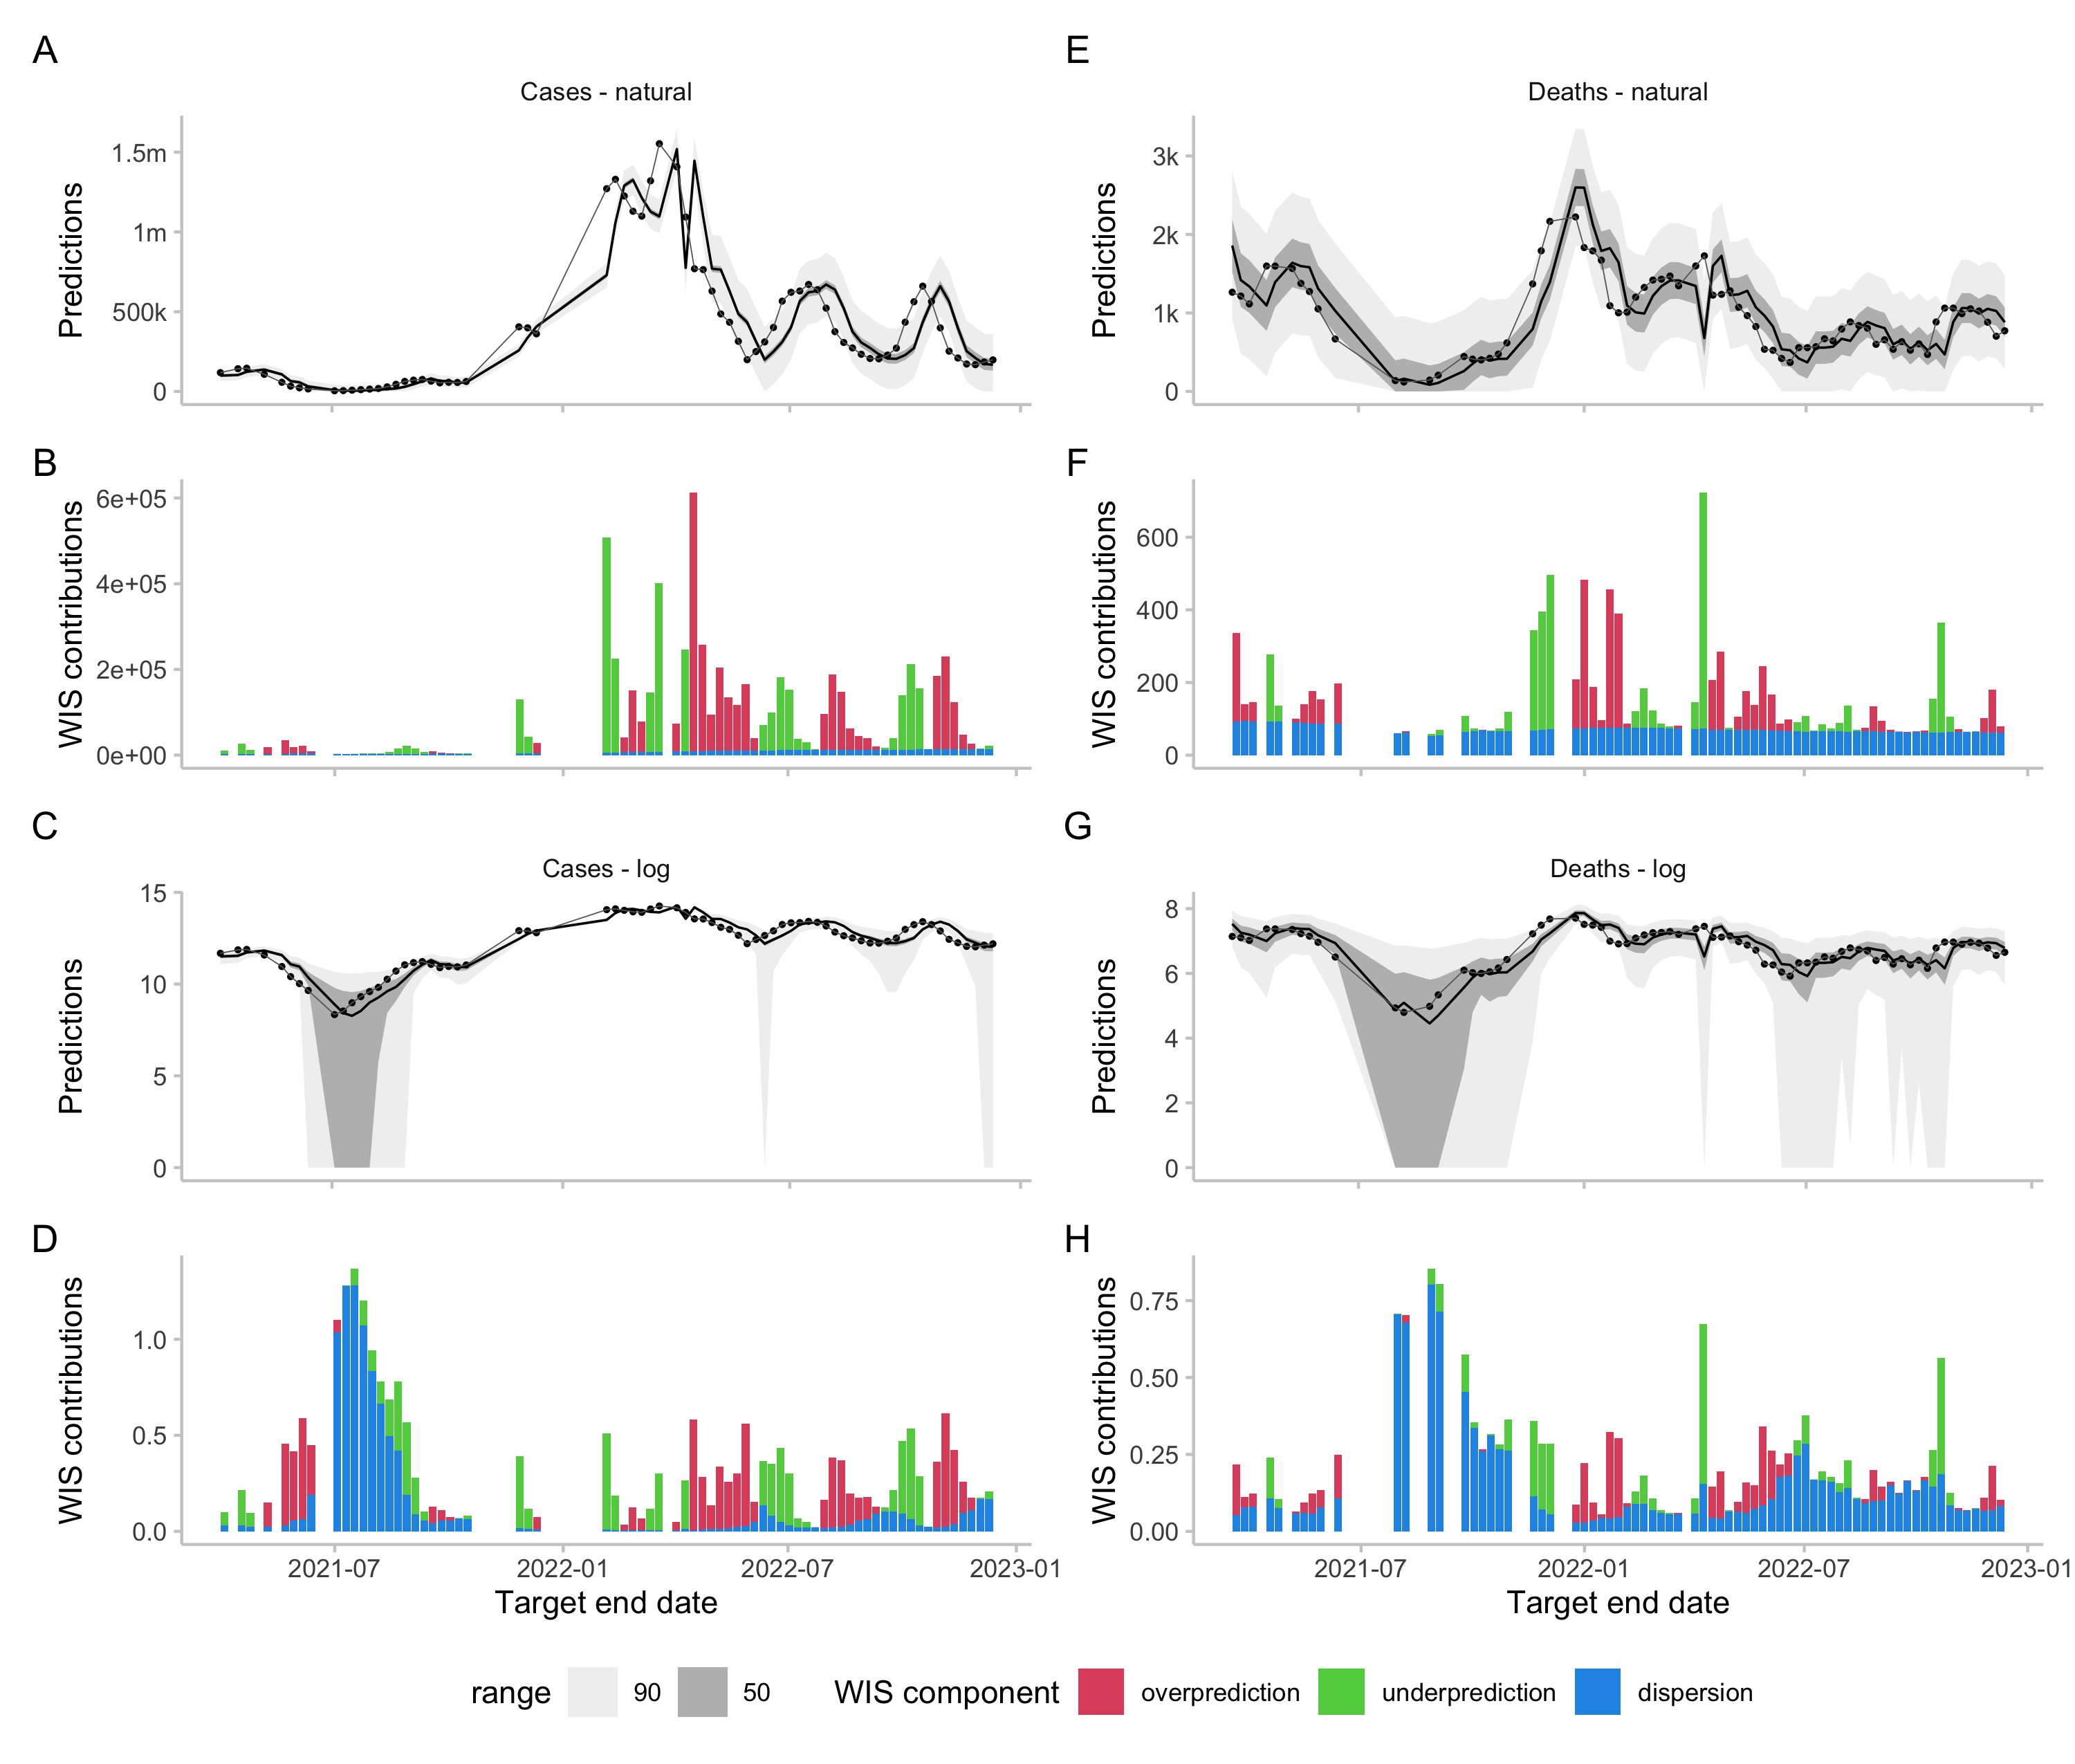
\includegraphics[width=0.99\textwidth]{output/figures/HUB-model-comparison-baseline.png}
    \caption{
    Forecasts and scores for two-week-ahead predictions from the EuroCOVIDhub-baseline made in Germany. The model had zero included in some of its 50 percent intervals (e.g. for case forecasts in July), leading to excessive dispersion values on the log scale. One could argue that including zero in the prediction intervals constituted an unreasonable forecast that was rightly penalised, but in general care has to be taken with small numbers. A, E: 50\% and 90\% prediction intervals and observed values for cases and deaths on the natural scale. B, F: Corresponding scores. C, G: Forecasts and observations on the log scale. D, H: Corresponding scores. 
    }
    \label{fig:HUB-model-comparison-baseline}
\end{figure}

\begin{figure}[h!]
    \centering
    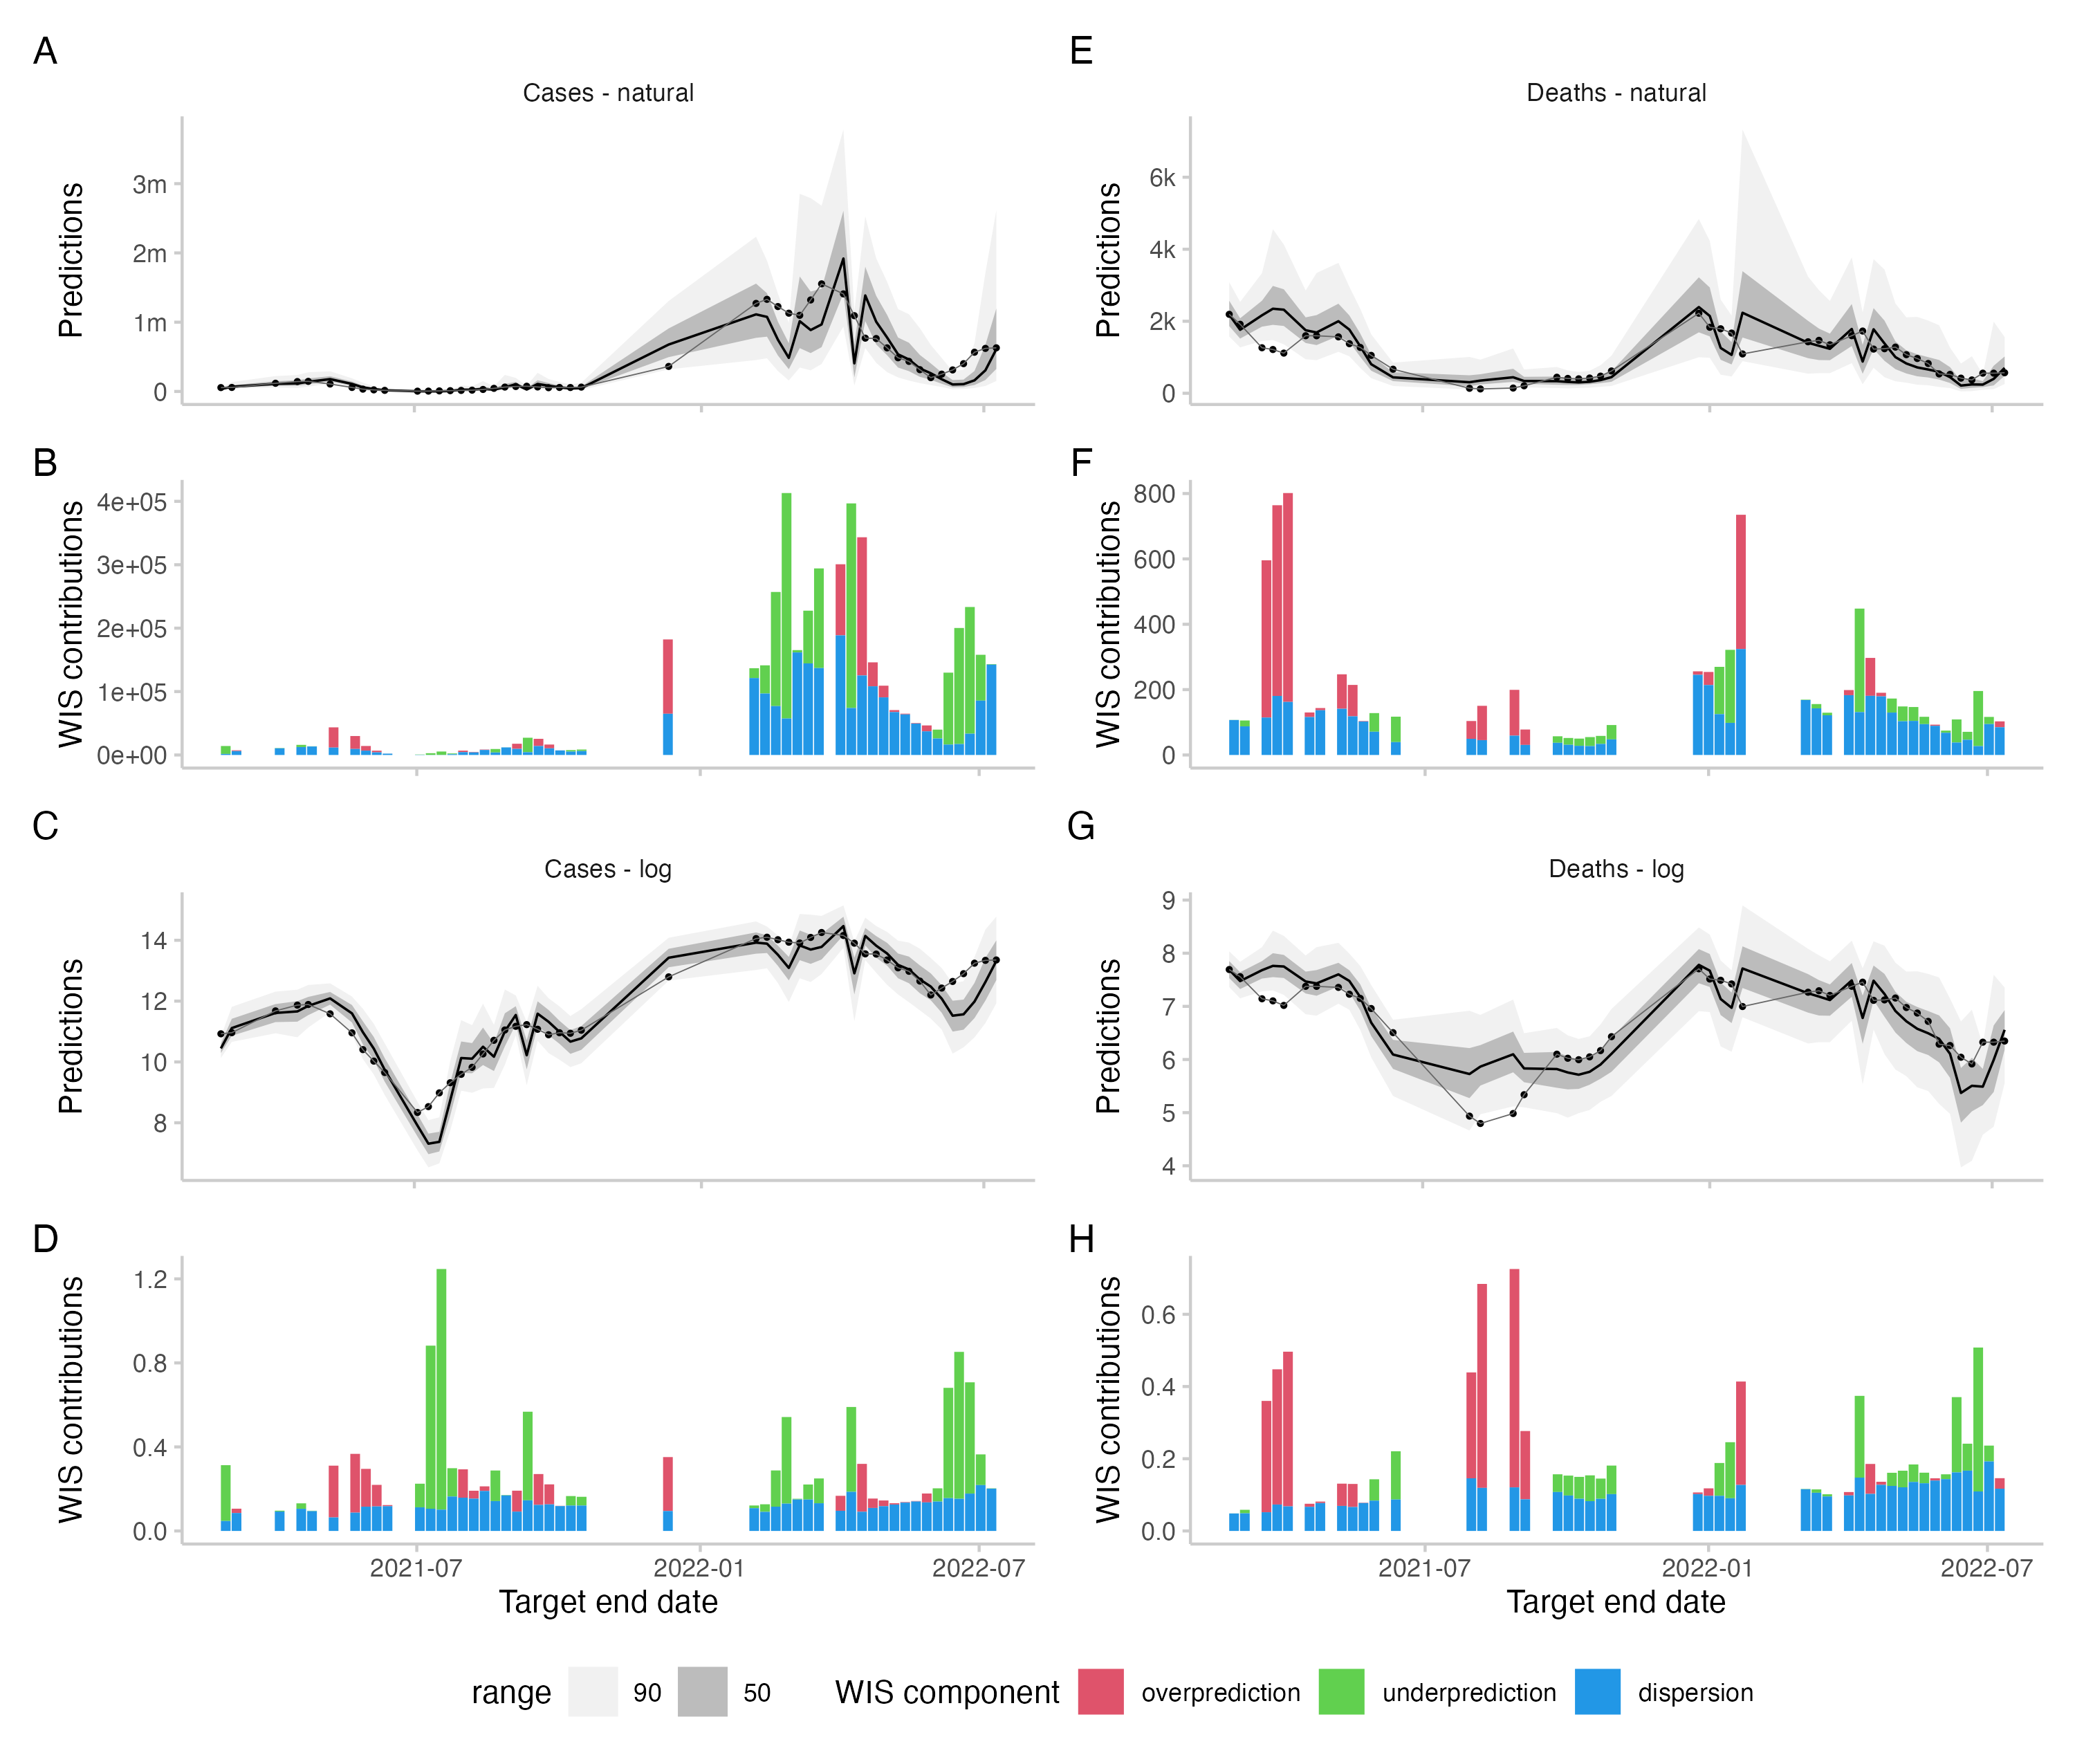
\includegraphics[width=0.99\textwidth]{output/figures/HUB-model-comparison-epinow.png}
    \caption{
    Forecasts and scores for two-week-ahead predictions from the epiforecasts-EpiNow2 model made in Germany. A, E: 50\% and 90\% prediction intervals and observed values for cases and deaths on the natural scale. B, F: Corresponding scores. C, G: Forecasts and observations on the log scale. D, H: Corresponding scores. 
    }
    \label{fig:HUB-model-comparison-epinow}
\end{figure}

\clearpage
\bibliography{log-or-not.bib}


\end{document}